%********************************************%
%*       Generated from PreTeXt source      *%
%*       on 2020-08-09T15:48:14-04:00       *%
%*   A recent stable commit (2020-07-07):   *%
%* 1771dacf84bfb1789139598d8379414b560b8f17 *%
%*                                          *%
%*         https://pretextbook.org          *%
%*                                          *%
%********************************************%
\documentclass[oneside,10pt,]{book}
%% Custom Preamble Entries, early (use latex.preamble.early)
%% Default LaTeX packages
%%   1.  always employed (or nearly so) for some purpose, or
%%   2.  a stylewriter may assume their presence
\usepackage{geometry}
%% Some aspects of the preamble are conditional,
%% the LaTeX engine is one such determinant
\usepackage{ifthen}
%% etoolbox has a variety of modern conveniences
\usepackage{etoolbox}
\usepackage{ifxetex,ifluatex}
%% Raster graphics inclusion
\usepackage{graphicx}
%% Color support, xcolor package
%% Always loaded, for: add/delete text, author tools
%% Here, since tcolorbox loads tikz, and tikz loads xcolor
\PassOptionsToPackage{usenames,dvipsnames,svgnames,table}{xcolor}
\usepackage{xcolor}
%% begin: defined colors, via xcolor package, for styling
%% end: defined colors, via xcolor package, for styling
%% Colored boxes, and much more, though mostly styling
%% skins library provides "enhanced" skin, employing tikzpicture
%% boxes may be configured as "breakable" or "unbreakable"
%% "raster" controls grids of boxes, aka side-by-side
\usepackage{tcolorbox}
\tcbuselibrary{skins}
\tcbuselibrary{breakable}
\tcbuselibrary{raster}
%% We load some "stock" tcolorbox styles that we use a lot
%% Placement here is provisional, there will be some color work also
%% First, black on white, no border, transparent, but no assumption about titles
\tcbset{ bwminimalstyle/.style={size=minimal, boxrule=-0.3pt, frame empty,
colback=white, colbacktitle=white, coltitle=black, opacityfill=0.0} }
%% Second, bold title, run-in to text/paragraph/heading
%% Space afterwards will be controlled by environment,
%% independent of constructions of the tcb title
%% Places \blocktitlefont onto many block titles
\tcbset{ runintitlestyle/.style={fonttitle=\blocktitlefont\upshape\bfseries, attach title to upper} }
%% Spacing prior to each exercise, anywhere
\tcbset{ exercisespacingstyle/.style={before skip={1.5ex plus 0.5ex}} }
%% Spacing prior to each block
\tcbset{ blockspacingstyle/.style={before skip={2.0ex plus 0.5ex}} }
%% xparse allows the construction of more robust commands,
%% this is a necessity for isolating styling and behavior
%% The tcolorbox library of the same name loads the base library
\tcbuselibrary{xparse}
%% Hyperref should be here, but likes to be loaded late
%%
%% Inline math delimiters, \(, \), need to be robust
%% 2016-01-31:  latexrelease.sty  supersedes  fixltx2e.sty
%% If  latexrelease.sty  exists, bugfix is in kernel
%% If not, bugfix is in  fixltx2e.sty
%% See:  https://tug.org/TUGboat/tb36-3/tb114ltnews22.pdf
%% and read "Fewer fragile commands" in distribution's  latexchanges.pdf
\IfFileExists{latexrelease.sty}{}{\usepackage{fixltx2e}}
%% Footnote counters and part/chapter counters are manipulated
%% April 2018:  chngcntr  commands now integrated into the kernel,
%% but circa 2018/2019 the package would still try to redefine them,
%% so we need to do the work of loading conditionally for old kernels.
%% From version 1.1a,  chngcntr  should detect defintions made by LaTeX kernel.
\ifdefined\counterwithin
\else
    \usepackage{chngcntr}
\fi
%% Text height identically 9 inches, text width varies on point size
%% See Bringhurst 2.1.1 on measure for recommendations
%% 75 characters per line (count spaces, punctuation) is target
%% which is the upper limit of Bringhurst's recommendations
\geometry{letterpaper,total={340pt,9.0in}}
%% Custom Page Layout Adjustments (use latex.geometry)
%% This LaTeX file may be compiled with pdflatex, xelatex, or lualatex executables
%% LuaTeX is not explicitly supported, but we do accept additions from knowledgeable users
%% The conditional below provides  pdflatex  specific configuration last
%% begin: engine-specific capabilities
\ifthenelse{\boolean{xetex} \or \boolean{luatex}}{%
%% begin: xelatex and lualatex-specific default configuration
\ifxetex\usepackage{xltxtra}\fi
%% realscripts is the only part of xltxtra relevant to lualatex 
\ifluatex\usepackage{realscripts}\fi
%% end:   xelatex and lualatex-specific default configuration
}{
%% begin: pdflatex-specific default configuration
%% We assume a PreTeXt XML source file may have Unicode characters
%% and so we ask LaTeX to parse a UTF-8 encoded file
%% This may work well for accented characters in Western language,
%% but not with Greek, Asian languages, etc.
%% When this is not good enough, switch to the  xelatex  engine
%% where Unicode is better supported (encouraged, even)
\usepackage[utf8]{inputenc}
%% end: pdflatex-specific default configuration
}
%% end:   engine-specific capabilities
%%
%% Fonts.  Conditional on LaTex engine employed.
%% Default Text Font: The Latin Modern fonts are
%% "enhanced versions of the [original TeX] Computer Modern fonts."
%% We use them as the default text font for PreTeXt output.
%% Automatic Font Control
%% Portions of a document, are, or may, be affected by defined commands
%% These are perhaps more flexible when using  xelatex  rather than  pdflatex
%% The following definitions are meant to be re-defined in a style, using \renewcommand
%% They are scoped when employed (in a TeX group), and so should not be defined with an argument
\newcommand{\divisionfont}{\relax}
\newcommand{\blocktitlefont}{\relax}
\newcommand{\contentsfont}{\relax}
\newcommand{\pagefont}{\relax}
\newcommand{\tabularfont}{\relax}
\newcommand{\xreffont}{\relax}
\newcommand{\titlepagefont}{\relax}
%%
\ifthenelse{\boolean{xetex} \or \boolean{luatex}}{%
%% begin: font setup and configuration for use with xelatex
%% Generally, xelatex is necessary for non-Western fonts
%% fontspec package provides extensive control of system fonts,
%% meaning *.otf (OpenType), and apparently *.ttf (TrueType)
%% that live *outside* your TeX/MF tree, and are controlled by your *system*
%% (it is possible that a TeX distribution will place fonts in a system location)
%%
%% The fontspec package is the best vehicle for using different fonts in  xelatex
%% So we load it always, no matter what a publisher or style might want
%%
\usepackage{fontspec}
%%
%% begin: xelatex main font ("font-xelatex-main" template)
%% Latin Modern Roman is the default font for xelatex and so is loaded with a TU encoding
%% *in the format* so we can't touch it, only perhaps adjust it later
%% in one of two ways (then known by NFSS names such as "lmr")
%% (1) via NFSS with font family names such as "lmr" and "lmss"
%% (2) via fontspec with commands like \setmainfont{Latin Modern Roman}
%% The latter requires the font to be known at the system-level by its font name,
%% but will give access to OTF font features through optional arguments
%% https://tex.stackexchange.com/questions/470008/
%% where-and-how-does-fontspec-sty-specify-the-default-font-latin-modern-roman
%% http://tex.stackexchange.com/questions/115321
%% /how-to-optimize-latin-modern-font-with-xelatex
%%
%% end:   xelatex main font ("font-xelatex-main" template)
%% begin: xelatex mono font ("font-xelatex-mono" template)
%% (conditional on non-trivial uses being present in source)
%% end:   xelatex mono font ("font-xelatex-mono" template)
%% begin: xelatex font adjustments ("font-xelatex-style" template)
%% end:   xelatex font adjustments ("font-xelatex-style" template)
%%
%% Extensive support for other languages
\usepackage{polyglossia}
%% Set main/default language based on pretext/@xml:lang value
%% document language code is "en-US", US English
%% usmax variant has extra hypenation
\setmainlanguage[variant=usmax]{english}
%% Enable secondary languages based on discovery of @xml:lang values
%% Enable fonts/scripts based on discovery of @xml:lang values
%% Western languages should be ably covered by Latin Modern Roman
%% end:   font setup and configuration for use with xelatex
}{%
%% begin: font setup and configuration for use with pdflatex
%% begin: pdflatex main font ("font-pdflatex-main" template)
\usepackage{lmodern}
\usepackage[T1]{fontenc}
%% end:   pdflatex main font ("font-pdflatex-main" template)
%% begin: pdflatex mono font ("font-pdflatex-mono" template)
%% (conditional on non-trivial uses being present in source)
%% end:   pdflatex mono font ("font-pdflatex-mono" template)
%% begin: pdflatex font adjustments ("font-pdflatex-style" template)
%% end:   pdflatex font adjustments ("font-pdflatex-style" template)
%% end:   font setup and configuration for use with pdflatex
}
%% Symbols, align environment, commutative diagrams, bracket-matrix
\usepackage{amsmath}
\usepackage{amscd}
\usepackage{amssymb}
%% allow page breaks within display mathematics anywhere
%% level 4 is maximally permissive
%% this is exactly the opposite of AMSmath package philosophy
%% there are per-display, and per-equation options to control this
%% split, aligned, gathered, and alignedat are not affected
\allowdisplaybreaks[4]
%% allow more columns to a matrix
%% can make this even bigger by overriding with  latex.preamble.late  processing option
\setcounter{MaxMatrixCols}{30}
%%
%%
%% Division Titles, and Page Headers/Footers
%% titlesec package, loading "titleps" package cooperatively
%% See code comments about the necessity and purpose of "explicit" option.
%% The "newparttoc" option causes a consistent entry for parts in the ToC 
%% file, but it is only effective if there is a \titleformat for \part.
%% "pagestyles" loads the  titleps  package cooperatively.
\usepackage[explicit, newparttoc, pagestyles]{titlesec}
%% The companion titletoc package for the ToC.
\usepackage{titletoc}
%% Fixes a bug with transition from chapters to appendices in a "book"
%% See generating XSL code for more details about necessity
\newtitlemark{\chaptertitlename}
%% begin: customizations of page styles via the modal "titleps-style" template
%% Designed to use commands from the LaTeX "titleps" package
%% Plain pages should have the same font for page numbers
\renewpagestyle{plain}{%
\setfoot{}{\pagefont\thepage}{}%
}%
%% Single pages as in default LaTeX
\renewpagestyle{headings}{%
\sethead{\pagefont\slshape\MakeUppercase{\ifthechapter{\chaptertitlename\space\thechapter.\space}{}\chaptertitle}}{}{\pagefont\thepage}%
}%
\pagestyle{headings}
%% end: customizations of page styles via the modal "titleps-style" template
%%
%% Create globally-available macros to be provided for style writers
%% These are redefined for each occurence of each division
\newcommand{\divisionnameptx}{\relax}%
\newcommand{\titleptx}{\relax}%
\newcommand{\subtitleptx}{\relax}%
\newcommand{\shortitleptx}{\relax}%
\newcommand{\authorsptx}{\relax}%
\newcommand{\epigraphptx}{\relax}%
%% Create environments for possible occurences of each division
%% Environment for a PTX "chapter" at the level of a LaTeX "chapter"
\NewDocumentEnvironment{chapterptx}{mmmmmm}
{%
\renewcommand{\divisionnameptx}{Chapter}%
\renewcommand{\titleptx}{#1}%
\renewcommand{\subtitleptx}{#2}%
\renewcommand{\shortitleptx}{#3}%
\renewcommand{\authorsptx}{#4}%
\renewcommand{\epigraphptx}{#5}%
\chapter[{#3}]{#1}%
\label{#6}%
}{}%
%% Environment for a PTX "section" at the level of a LaTeX "section"
\NewDocumentEnvironment{sectionptx}{mmmmmm}
{%
\renewcommand{\divisionnameptx}{Section}%
\renewcommand{\titleptx}{#1}%
\renewcommand{\subtitleptx}{#2}%
\renewcommand{\shortitleptx}{#3}%
\renewcommand{\authorsptx}{#4}%
\renewcommand{\epigraphptx}{#5}%
\section[{#3}]{#1}%
\label{#6}%
}{}%
%% Environment for a PTX "worksheet" at the level of a LaTeX "subsection"
\NewDocumentEnvironment{worksheet-subsection}{mmmmmm}
{%
\renewcommand{\divisionnameptx}{Worksheet}%
\renewcommand{\titleptx}{#1}%
\renewcommand{\subtitleptx}{#2}%
\renewcommand{\shortitleptx}{#3}%
\renewcommand{\authorsptx}{#4}%
\renewcommand{\epigraphptx}{#5}%
\subsection[{#3}]{#1}%
\label{#6}%
}{}%
%% Environment for a PTX "worksheet" at the level of a LaTeX "subsection"
\NewDocumentEnvironment{worksheet-subsection-numberless}{mmmmmm}
{%
\renewcommand{\divisionnameptx}{Worksheet}%
\renewcommand{\titleptx}{#1}%
\renewcommand{\subtitleptx}{#2}%
\renewcommand{\shortitleptx}{#3}%
\renewcommand{\authorsptx}{#4}%
\renewcommand{\epigraphptx}{#5}%
\subsection*{#1}%
\addcontentsline{toc}{subsection}{#3}
\label{#6}%
}{}%
%%
%% Styles for six traditional LaTeX divisions
\titleformat{\part}[display]
{\divisionfont\Huge\bfseries\centering}{\divisionnameptx\space\thepart}{30pt}{\Huge#1}
[{\Large\centering\authorsptx}]
\titleformat{\chapter}[display]
{\divisionfont\huge\bfseries}{\divisionnameptx\space\thechapter}{20pt}{\Huge#1}
[{\Large\authorsptx}]
\titleformat{name=\chapter,numberless}[display]
{\divisionfont\huge\bfseries}{}{0pt}{#1}
[{\Large\authorsptx}]
\titlespacing*{\chapter}{0pt}{50pt}{40pt}
\titleformat{\section}[hang]
{\divisionfont\Large\bfseries}{\thesection}{1ex}{#1}
[{\large\authorsptx}]
\titleformat{name=\section,numberless}[block]
{\divisionfont\Large\bfseries}{}{0pt}{#1}
[{\large\authorsptx}]
\titlespacing*{\section}{0pt}{3.5ex plus 1ex minus .2ex}{2.3ex plus .2ex}
\titleformat{\subsection}[hang]
{\divisionfont\large\bfseries}{\thesubsection}{1ex}{#1}
[{\normalsize\authorsptx}]
\titleformat{name=\subsection,numberless}[block]
{\divisionfont\large\bfseries}{}{0pt}{#1}
[{\normalsize\authorsptx}]
\titlespacing*{\subsection}{0pt}{3.25ex plus 1ex minus .2ex}{1.5ex plus .2ex}
\titleformat{\subsubsection}[hang]
{\divisionfont\normalsize\bfseries}{\thesubsubsection}{1em}{#1}
[{\small\authorsptx}]
\titleformat{name=\subsubsection,numberless}[block]
{\divisionfont\normalsize\bfseries}{}{0pt}{#1}
[{\normalsize\authorsptx}]
\titlespacing*{\subsubsection}{0pt}{3.25ex plus 1ex minus .2ex}{1.5ex plus .2ex}
\titleformat{\paragraph}[hang]
{\divisionfont\normalsize\bfseries}{\theparagraph}{1em}{#1}
[{\small\authorsptx}]
\titleformat{name=\paragraph,numberless}[block]
{\divisionfont\normalsize\bfseries}{}{0pt}{#1}
[{\normalsize\authorsptx}]
\titlespacing*{\paragraph}{0pt}{3.25ex plus 1ex minus .2ex}{1.5em}
%%
%% Styles for five traditional LaTeX divisions
\titlecontents{part}%
[0pt]{\contentsmargin{0em}\addvspace{1pc}\contentsfont\bfseries}%
{\Large\thecontentslabel\enspace}{\Large}%
{}%
[\addvspace{.5pc}]%
\titlecontents{chapter}%
[0pt]{\contentsmargin{0em}\addvspace{1pc}\contentsfont\bfseries}%
{\large\thecontentslabel\enspace}{\large}%
{\hfill\bfseries\thecontentspage}%
[\addvspace{.5pc}]%
\dottedcontents{section}[3.8em]{\contentsfont}{2.3em}{1pc}%
\dottedcontents{subsection}[6.1em]{\contentsfont}{3.2em}{1pc}%
\dottedcontents{subsubsection}[9.3em]{\contentsfont}{4.3em}{1pc}%
%%
%% Begin: Semantic Macros
%% To preserve meaning in a LaTeX file
%%
%% \mono macro for content of "c", "cd", "tag", etc elements
%% Also used automatically in other constructions
%% Simply an alias for \texttt
%% Always defined, even if there is no need, or if a specific tt font is not loaded
\newcommand{\mono}[1]{\texttt{#1}}
%%
%% Following semantic macros are only defined here if their
%% use is required only in this specific document
%%
%% End: Semantic Macros
%% Division Numbering: Chapters, Sections, Subsections, etc
%% Division numbers may be turned off at some level ("depth")
%% A section *always* has depth 1, contrary to us counting from the document root
%% The latex default is 3.  If a larger number is present here, then
%% removing this command may make some cross-references ambiguous
%% The precursor variable $numbering-maxlevel is checked for consistency in the common XSL file
\setcounter{secnumdepth}{3}
%%
%% AMS "proof" environment is no longer used, but we leave previously
%% implemented \qedhere in place, should the LaTeX be recycled
\newcommand{\qedhere}{\relax}
%%
%% A faux tcolorbox whose only purpose is to provide common numbering
%% facilities for most blocks (possibly not projects, 2D displays)
%% Controlled by  numbering.theorems.level  processing parameter
\newtcolorbox[auto counter, number within=section]{block}{}
%%
%% This document is set to number PROJECT-LIKE on a separate numbering scheme
%% So, a faux tcolorbox whose only purpose is to provide this numbering
%% Controlled by  numbering.projects.level  processing parameter
\newtcolorbox[auto counter, number within=section]{project-distinct}{}
%% A faux tcolorbox whose only purpose is to provide common numbering
%% facilities for 2D displays which are subnumbered as part of a "sidebyside"
\newtcolorbox[auto counter, number within=tcb@cnt@block, number freestyle={\noexpand\thetcb@cnt@block(\noexpand\alph{\tcbcounter})}]{subdisplay}{}
%% Divisional exercises (and worksheet) as LaTeX environments
%% Third argument is option for extra workspace in worksheets
%% Hanging indent occupies a 5ex width slot prior to left margin
%% Experimentally this seems just barely sufficient for a bold "888."
%% Division exercises, not in exercise group
\tcbset{ divisionexercisestyle/.style={bwminimalstyle, runintitlestyle, exercisespacingstyle, left=5ex, breakable, parbox=false } }
\newtcolorbox{divisionexercise}[4]{divisionexercisestyle, before title={\hspace{-5ex}\makebox[5ex][l]{#1.}}, title={\notblank{#2}{#2\space}{}}, phantom={\hypertarget{#4}{}}, after={\notblank{#3}{\newline\rule{\workspacestrutwidth}{#3\textheight}\newline}{}}}
%% Localize LaTeX supplied names (possibly none)
\renewcommand*{\chaptername}{Chapter}
%% Equation Numbering
%% Controlled by  numbering.equations.level  processing parameter
%% No adjustment here implies document-wide numbering
\numberwithin{equation}{section}
%% "tcolorbox" environment for a single image, occupying entire \linewidth
%% arguments are left-margin, width, right-margin, as multiples of
%% \linewidth, and are guaranteed to be positive and sum to 1.0
\tcbset{ imagestyle/.style={bwminimalstyle} }
\NewTColorBox{image}{mmm}{imagestyle,left skip=#1\linewidth,width=#2\linewidth}
%% Footnote Numbering
%% Specified by numbering.footnotes.level
%% Undo counter reset by chapter for a book
\counterwithout{footnote}{chapter}
\counterwithin*{footnote}{section}
%% QR Code Support
%% Videos and other interactives
\usepackage{qrcode}
\newlength{\qrsize}
\newlength{\previewwidth}
%% tcolorbox styles for interactive previews
%% changing size= and/or colback can aid in debugging
\tcbset{ previewstyle/.style={bwminimalstyle, halign=center} }
\tcbset{ qrstyle/.style={bwminimalstyle, hbox} }
\tcbset{ captionstyle/.style={bwminimalstyle, left=1em, width=\linewidth} }
%% Generic red play button (from SVG)
%% tikz package should be loaded by now
\definecolor{playred}{RGB}{230,33,23}
\newcommand{\genericpreview}{
        
\begin{tikzpicture}[y=0.80pt, x=0.80pt, yscale=-1.000000, xscale=1.000000, inner sep=0pt, outer sep=0pt]
        \path[fill=playred] (94.9800,28.8400) .. controls (94.9800,28.8400) and
        (94.0400,22.2400) .. (91.1700,19.3400) .. controls (87.5300,15.5300) and
        (83.4500,15.5100) .. (81.5800,15.2900) .. controls (68.1800,14.3200) and
        (48.0600,14.4400) .. (48.0600,14.4400) .. controls (48.0600,14.4400) and
        (27.9400,14.3200) .. (14.5400,15.2900) .. controls (12.6700,15.5100) and
        (8.5900,15.5300) .. (4.9500,19.3400) .. controls (2.0800,22.2400) and
        (1.1400,28.8400) .. (1.1400,28.8400) .. controls (1.1400,28.8400) and
        (0.1800,36.5800) .. (0.0000,44.3300) -- (0.0000,51.5900) .. controls
        (0.1800,59.3400) and (1.1400,67.0800) .. (1.1400,67.0800) .. controls
        (1.1400,67.0800) and (2.0700,73.6800) .. (4.9500,76.5800) .. controls
        (8.5900,80.3900) and (13.3800,80.2700) .. (15.5100,80.6700) .. controls
        (23.0400,81.3900) and (47.2100,81.5600) .. (48.0500,81.5700) .. controls
        (48.0600,81.5700) and (68.1900,81.6000) .. (81.5900,80.6300) .. controls
        (83.4600,80.4100) and (87.5400,80.3900) .. (91.1800,76.5800) .. controls
        (94.0500,73.6800) and (94.9900,67.0800) .. (94.9900,67.0800) .. controls
        (94.9900,67.0800) and (95.9500,59.3300) .. (96.0100,51.5900) --
        (96.0100,44.3300) .. controls (95.9400,36.5800) and (94.9800,28.8400) ..
        (94.9800,28.8400) -- cycle(38.2800,61.4100) -- (38.2800,34.4100) --
        (64.0200,47.9100) -- (38.2800,61.4100) -- cycle;
        \end{tikzpicture}
        }
%% More flexible list management, esp. for references
%% But also for specifying labels (i.e. custom order) on nested lists
\usepackage{enumitem}
%% hyperref driver does not need to be specified, it will be detected
%% Footnote marks in tcolorbox have broken linking under
%% hyperref, so it is necessary to turn off all linking
%% It *must* be given as a package option, not with \hypersetup
\usepackage[hyperfootnotes=false]{hyperref}
%% Hyperlinking active in electronic PDFs, all links solid and blue
\hypersetup{colorlinks=true,linkcolor=blue,citecolor=blue,filecolor=blue,urlcolor=blue}
\hypersetup{pdftitle={MATH 140 Summer 2020}}
%% If you manually remove hyperref, leave in this next command
\providecommand\phantomsection{}
%% If tikz has been loaded, replace ampersand with \amp macro
%% extpfeil package for certain extensible arrows,
%% as also provided by MathJax extension of the same name
%% NB: this package loads mtools, which loads calc, which redefines
%%     \setlength, so it can be removed if it seems to be in the 
%%     way and your math does not use:
%%     
%%     \xtwoheadrightarrow, \xtwoheadleftarrow, \xmapsto, \xlongequal, \xtofrom
%%     
%%     we have had to be extra careful with variable thickness
%%     lines in tables, and so also load this package late
\usepackage{extpfeil}
%% Custom Preamble Entries, late (use latex.preamble.late)
%% Begin: Author-provided packages
%% (From  docinfo/latex-preamble/package  elements)
%% End: Author-provided packages
%% Begin: Author-provided macros
%% (From  docinfo/macros  element)
%% Plus three from MBX for XML characters
\newcommand{\doubler}[1]{2#1}
\newcommand{\lt}{<}
\newcommand{\gt}{>}
\newcommand{\amp}{&}
%% End: Author-provided macros
\begin{document}
\frontmatter
%% begin: half-title
\thispagestyle{empty}
{\titlepagefont\centering
\vspace*{0.28\textheight}
{\Huge MATH 140 Summer 2020}\\}
\clearpage
%% end:   half-title
%% begin: adcard
\thispagestyle{empty}
\null%
\clearpage
%% end:   adcard
%% begin: title page
%% Inspired by Peter Wilson's "titleDB" in "titlepages" CTAN package
\thispagestyle{empty}
{\titlepagefont\centering
\vspace*{0.14\textheight}
%% Target for xref to top-level element is ToC
\addtocontents{toc}{\protect\hypertarget{x:book:Math140Summer2020}{}}
{\Huge MATH 140 Summer 2020}\\[3\baselineskip]
{\Large Daniel Moseley}\\[0.5\baselineskip]
{\Large Jacksonville University}\\[3\baselineskip]
{\Large August 9, 2020}\\}
\clearpage
%% end:   title page
%% begin: copyright-page
\thispagestyle{empty}
\vspace*{\stretch{2}}
\vspace*{\stretch{1}}
\null\clearpage
%% end:   copyright-page
\setlength{\qrsize}{9em}
\setlength{\previewwidth}{\linewidth}
\addtolength{\previewwidth}{-\qrsize}
\begin{tcbraster}[raster columns=2, raster column skip=1pt, raster halign=center, raster force size=false, raster left skip=0pt, raster right skip=0pt]%
\begin{tcolorbox}[previewstyle, width=\previewwidth]%
\includegraphics[width=0.80\linewidth,height=\qrsize,keepaspectratio]{images/video-1.jpg}%
\end{tcolorbox}%
\begin{tcolorbox}[qrstyle]%
{\hypersetup{urlcolor=black}\qrcode[height=\qrsize]{https://www.youtube.com/watch?v=u7gLANu3-Yo}}%
\end{tcolorbox}%
\begin{tcolorbox}[captionstyle]%
\small YouTube: \mono{https://www.youtube.com/watch?v=u7gLANu3-Yo}\end{tcolorbox}%
\end{tcbraster}%
This is a collection of the materials (outside of the textbook) we will use in class to guide you on your journey through MATH 140. The textbook used in the course will be Calculus: Single Variable, 7th Edition edition by Hughes-Hallett, et al.%
%% begin: table of contents
%% Adjust Table of Contents
\setcounter{tocdepth}{1}
\renewcommand*\contentsname{Contents}
\tableofcontents
%% end:   table of contents
\mainmatter
This is a collection of the materials (outside of the textbook) we will use in class to guide you on your journey through MATH 140.%
%
%
\typeout{************************************************}
\typeout{Chapter 1 Week 1 - Limits and Speed}
\typeout{************************************************}
%
\begin{chapterptx}{Week 1 - Limits and Speed}{}{Week 1 - Limits and Speed}{}{}{x:chapter:week1}
%
%
\typeout{************************************************}
\typeout{Section 1.1 Section 1.7 - Introduction to Continuity and Limits}
\typeout{************************************************}
%
\begin{sectionptx}{Section 1.7 - Introduction to Continuity and Limits}{}{Section 1.7 - Introduction to Continuity and Limits}{}{}{x:section:section1_7}
\setlength{\qrsize}{9em}
\setlength{\previewwidth}{\linewidth}
\addtolength{\previewwidth}{-\qrsize}
\begin{tcbraster}[raster columns=2, raster column skip=1pt, raster halign=center, raster force size=false, raster left skip=0pt, raster right skip=0pt]%
\begin{tcolorbox}[previewstyle, width=\previewwidth]%
\includegraphics[width=0.80\linewidth,height=\qrsize,keepaspectratio]{images/video-2.jpg}%
\end{tcolorbox}%
\begin{tcolorbox}[qrstyle]%
{\hypersetup{urlcolor=black}\qrcode[height=\qrsize]{https://www.youtube.com/watch?v=h3khNZKCZPA}}%
\end{tcolorbox}%
\begin{tcolorbox}[captionstyle]%
\small YouTube: \mono{https://www.youtube.com/watch?v=h3khNZKCZPA}\end{tcolorbox}%
\end{tcbraster}%
%
%
\typeout{************************************************}
\typeout{Worksheet 1.1.1 Worksheet}
\typeout{************************************************}
%
\newgeometry{left=1.25cm, right=1.25cm, top=1.25cm, bottom=1.25cm}
\begin{worksheet-subsection}{Worksheet}{}{Worksheet}{}{}{g:worksheet:idm389855657968}
\begin{divisionexercise}{1}{}{}{g:exercise:idm389855659584}%
Are the following functions continuous?%
%
\begin{enumerate}[label=(\alph*)]
\item{}%
\begin{equation*}
f(x) = \left\{ \begin{matrix} x & x \leq 1 \\ x^2 & x > 1 \end{matrix} \right. 
\end{equation*}
%
\item{}%
\begin{equation*}
g(x) = \left\{ \begin{matrix} \frac x{\left\vert x \right\vert} & x \neq 0 \\ 0 & x = 0 \end{matrix} \right. 
\end{equation*}
%
\end{enumerate}
\setlength{\qrsize}{9em}
\setlength{\previewwidth}{\linewidth}
\addtolength{\previewwidth}{-\qrsize}
\begin{tcbraster}[raster columns=2, raster column skip=1pt, raster halign=center, raster force size=false, raster left skip=0pt, raster right skip=0pt]%
\begin{tcolorbox}[previewstyle, width=\previewwidth]%
\IfFileExists{images/interactive-1-preview.png}%
{\includegraphics[width=0.80\linewidth,height=\qrsize,keepaspectratio]{images/interactive-1-preview.png}}%
{\small{}Specify static image with \mono{@preview} attribute,\\Or create and provide automatic screenshot as \mono{images/interactive-1-preview.png} via the \mono{mbx} script}%
\end{tcolorbox}%
\begin{tcolorbox}[qrstyle]%
{\hypersetup{urlcolor=black}\qrcode[height=\qrsize]{/interactive-1.html}}%
\end{tcolorbox}%
\begin{tcolorbox}[captionstyle]%
\small \mono{www.desmos.com/calculator/}\end{tcolorbox}%
\end{tcbraster}%
%
\textbf{\blocktitlefont Solution}.\hypertarget{g:solution:idm389855675040}{}\quad{}%
\begin{enumerate}[label=(\alph*)]
\item{}Yes, it is continuous%
\par
\setlength{\qrsize}{9em}
\setlength{\previewwidth}{\linewidth}
\addtolength{\previewwidth}{-\qrsize}
\begin{tcbraster}[raster columns=2, raster column skip=1pt, raster halign=center, raster force size=false, raster left skip=0pt, raster right skip=0pt]%
\begin{tcolorbox}[previewstyle, width=\previewwidth]%
\IfFileExists{images/interactive-2-preview.png}%
{\includegraphics[width=0.80\linewidth,height=\qrsize,keepaspectratio]{images/interactive-2-preview.png}}%
{\small{}Specify static image with \mono{@preview} attribute,\\Or create and provide automatic screenshot as \mono{images/interactive-2-preview.png} via the \mono{mbx} script}%
\end{tcolorbox}%
\begin{tcolorbox}[qrstyle]%
{\hypersetup{urlcolor=black}\qrcode[height=\qrsize]{/interactive-2.html}}%
\end{tcolorbox}%
\begin{tcolorbox}[captionstyle]%
\small \mono{www.desmos.com/calculator/kslwpjxdgf}\end{tcolorbox}%
\end{tcbraster}%
%
\item{}No, it is not continuous%
\par
\setlength{\qrsize}{9em}
\setlength{\previewwidth}{\linewidth}
\addtolength{\previewwidth}{-\qrsize}
\begin{tcbraster}[raster columns=2, raster column skip=1pt, raster halign=center, raster force size=false, raster left skip=0pt, raster right skip=0pt]%
\begin{tcolorbox}[previewstyle, width=\previewwidth]%
\IfFileExists{images/interactive-3-preview.png}%
{\includegraphics[width=0.80\linewidth,height=\qrsize,keepaspectratio]{images/interactive-3-preview.png}}%
{\small{}Specify static image with \mono{@preview} attribute,\\Or create and provide automatic screenshot as \mono{images/interactive-3-preview.png} via the \mono{mbx} script}%
\end{tcolorbox}%
\begin{tcolorbox}[qrstyle]%
{\hypersetup{urlcolor=black}\qrcode[height=\qrsize]{/interactive-3.html}}%
\end{tcolorbox}%
\begin{tcolorbox}[captionstyle]%
\small \mono{www.desmos.com/calculator/emzeyduwy7}\end{tcolorbox}%
\end{tcbraster}%
%
\end{enumerate}
\end{divisionexercise}%
\begin{divisionexercise}{2}{}{}{g:exercise:idm389855690000}%
Find \(k\) so that the following function is continuous on any interval:%
\begin{equation*}
f(x) = \left \{ \begin{matrix} kx & x \leq 3 \\ 5 & x > 3 \end{matrix} \right. 
\end{equation*}
%
\par
\setlength{\qrsize}{9em}
\setlength{\previewwidth}{\linewidth}
\addtolength{\previewwidth}{-\qrsize}
\begin{tcbraster}[raster columns=2, raster column skip=1pt, raster halign=center, raster force size=false, raster left skip=0pt, raster right skip=0pt]%
\begin{tcolorbox}[previewstyle, width=\previewwidth]%
\IfFileExists{images/interactive-4-preview.png}%
{\includegraphics[width=0.80\linewidth,height=\qrsize,keepaspectratio]{images/interactive-4-preview.png}}%
{\small{}Specify static image with \mono{@preview} attribute,\\Or create and provide automatic screenshot as \mono{images/interactive-4-preview.png} via the \mono{mbx} script}%
\end{tcolorbox}%
\begin{tcolorbox}[qrstyle]%
{\hypersetup{urlcolor=black}\qrcode[height=\qrsize]{/interactive-4.html}}%
\end{tcolorbox}%
\begin{tcolorbox}[captionstyle]%
\small \mono{www.desmos.com/calculator/}\end{tcolorbox}%
\end{tcbraster}%
%
\textbf{\blocktitlefont Solution}.\hypertarget{g:solution:idm389855717648}{}\quad{}While I use Desmos for intuition, to find the exact answer we need the left and right sides to meet when \(x=3\). Thus we need \(k(3)=5\) and hence \(k=\frac 53\).%
\par
\setlength{\qrsize}{9em}
\setlength{\previewwidth}{\linewidth}
\addtolength{\previewwidth}{-\qrsize}
\begin{tcbraster}[raster columns=2, raster column skip=1pt, raster halign=center, raster force size=false, raster left skip=0pt, raster right skip=0pt]%
\begin{tcolorbox}[previewstyle, width=\previewwidth]%
\IfFileExists{images/interactive-5-preview.png}%
{\includegraphics[width=0.80\linewidth,height=\qrsize,keepaspectratio]{images/interactive-5-preview.png}}%
{\small{}Specify static image with \mono{@preview} attribute,\\Or create and provide automatic screenshot as \mono{images/interactive-5-preview.png} via the \mono{mbx} script}%
\end{tcolorbox}%
\begin{tcolorbox}[qrstyle]%
{\hypersetup{urlcolor=black}\qrcode[height=\qrsize]{/interactive-5.html}}%
\end{tcolorbox}%
\begin{tcolorbox}[captionstyle]%
\small \mono{www.desmos.com/calculator/v2lspd0dbo}\end{tcolorbox}%
\end{tcbraster}%
%
\end{divisionexercise}%
\begin{divisionexercise}{3}{}{}{g:exercise:idm389855716864}%
Let%
\begin{equation*}
f(x) = \frac{e^x - 1}{x}. 
\end{equation*}
%
%
\begin{enumerate}[label=(\alph*)]
\item{}Make a table of values of \(f(x)\) for \(x=0.1,0.01,0.001,0.0001,-0.1,-0.01,-0.001,-0.0001\).%
\item{}Make a conjecture (educated guess) about the value of%
\begin{equation*}
\lim _{x\to 0} f(x) .
\end{equation*}
%
\item{}Graph the function on your graphing calculator to see if it verifies your conjecture from parts a) and b).%
\end{enumerate}
\setlength{\qrsize}{9em}
\setlength{\previewwidth}{\linewidth}
\addtolength{\previewwidth}{-\qrsize}
\begin{tcbraster}[raster columns=2, raster column skip=1pt, raster halign=center, raster force size=false, raster left skip=0pt, raster right skip=0pt]%
\begin{tcolorbox}[previewstyle, width=\previewwidth]%
\IfFileExists{images/interactive-6-preview.png}%
{\includegraphics[width=0.80\linewidth,height=\qrsize,keepaspectratio]{images/interactive-6-preview.png}}%
{\small{}Specify static image with \mono{@preview} attribute,\\Or create and provide automatic screenshot as \mono{images/interactive-6-preview.png} via the \mono{mbx} script}%
\end{tcolorbox}%
\begin{tcolorbox}[qrstyle]%
{\hypersetup{urlcolor=black}\qrcode[height=\qrsize]{/interactive-6.html}}%
\end{tcolorbox}%
\begin{tcolorbox}[captionstyle]%
\small \mono{www.desmos.com/calculator/}\end{tcolorbox}%
\end{tcbraster}%
%
\textbf{\blocktitlefont Solution}.\hypertarget{g:solution:idm389855760480}{}\quad{}We see from both the table and the graph that \(f(x)\) approaches 1 as \(x\) approaches 0. Hence,%
\begin{equation*}
\lim_{x\to 0} f(x)=1
\end{equation*}
%
\par
\setlength{\qrsize}{9em}
\setlength{\previewwidth}{\linewidth}
\addtolength{\previewwidth}{-\qrsize}
\begin{tcbraster}[raster columns=2, raster column skip=1pt, raster halign=center, raster force size=false, raster left skip=0pt, raster right skip=0pt]%
\begin{tcolorbox}[previewstyle, width=\previewwidth]%
\IfFileExists{images/interactive-7-preview.png}%
{\includegraphics[width=0.80\linewidth,height=\qrsize,keepaspectratio]{images/interactive-7-preview.png}}%
{\small{}Specify static image with \mono{@preview} attribute,\\Or create and provide automatic screenshot as \mono{images/interactive-7-preview.png} via the \mono{mbx} script}%
\end{tcolorbox}%
\begin{tcolorbox}[qrstyle]%
{\hypersetup{urlcolor=black}\qrcode[height=\qrsize]{/interactive-7.html}}%
\end{tcolorbox}%
\begin{tcolorbox}[captionstyle]%
\small \mono{www.desmos.com/calculator/zswsdqkoct}\end{tcolorbox}%
\end{tcbraster}%
%
\end{divisionexercise}%
\end{worksheet-subsection}
\restoregeometry
\setlength{\qrsize}{9em}
\setlength{\previewwidth}{\linewidth}
\addtolength{\previewwidth}{-\qrsize}
\begin{tcbraster}[raster columns=2, raster column skip=1pt, raster halign=center, raster force size=false, raster left skip=0pt, raster right skip=0pt]%
\begin{tcolorbox}[previewstyle, width=\previewwidth]%
\includegraphics[width=0.80\linewidth,height=\qrsize,keepaspectratio]{images/video-3.jpg}%
\end{tcolorbox}%
\begin{tcolorbox}[qrstyle]%
{\hypersetup{urlcolor=black}\qrcode[height=\qrsize]{https://www.youtube.com/watch?v=oGegwwgPeXQ}}%
\end{tcolorbox}%
\begin{tcolorbox}[captionstyle]%
\small YouTube: \mono{https://www.youtube.com/watch?v=oGegwwgPeXQ}\end{tcolorbox}%
\end{tcbraster}%
\end{sectionptx}
%
%
\typeout{************************************************}
\typeout{Section 1.2 Section 1.8 - Extending the Idea of a Limit}
\typeout{************************************************}
%
\begin{sectionptx}{Section 1.8 - Extending the Idea of a Limit}{}{Section 1.8 - Extending the Idea of a Limit}{}{}{x:section:section1_8}
\setlength{\qrsize}{9em}
\setlength{\previewwidth}{\linewidth}
\addtolength{\previewwidth}{-\qrsize}
\begin{tcbraster}[raster columns=2, raster column skip=1pt, raster halign=center, raster force size=false, raster left skip=0pt, raster right skip=0pt]%
\begin{tcolorbox}[previewstyle, width=\previewwidth]%
\includegraphics[width=0.80\linewidth,height=\qrsize,keepaspectratio]{images/video-4.jpg}%
\end{tcolorbox}%
\begin{tcolorbox}[qrstyle]%
{\hypersetup{urlcolor=black}\qrcode[height=\qrsize]{https://www.youtube.com/watch?v=Y_LSb1botCA}}%
\end{tcolorbox}%
\begin{tcolorbox}[captionstyle]%
\small YouTube: \mono{https://www.youtube.com/watch?v=Y\_LSb1botCA}\end{tcolorbox}%
\end{tcbraster}%
%
%
\typeout{************************************************}
\typeout{Worksheet 1.2.1 Worksheet}
\typeout{************************************************}
%
\newgeometry{left=1.25cm, right=1.25cm, top=1.25cm, bottom=1.25cm}
\begin{worksheet-subsection}{Worksheet}{}{Worksheet}{}{}{g:worksheet:idm389855798224}
\begin{divisionexercise}{1}{}{}{g:exercise:idm389855800000}%
Compute%
\begin{equation*}
\lim_{x\to \infty} \frac{4x+5}{6x^2+7x+8}
\end{equation*}
%
\textbf{\blocktitlefont Solution}.\hypertarget{g:solution:idm389855800928}{}\quad{}You can evaluate this graphically, but to me the best tactic is to divide the numerator and denominator by the largest power of \(x\). In this case that is \(x^2\).%
\begin{equation*}
\lim_{x\to \infty} \frac{4x+5}{6x^2+7x+8} = \lim_{x\to \infty} \frac{\frac4x+\frac5{x^2}}{6+\frac7x+\frac8{x^2}} = 0 
\end{equation*}
Note that everything in the numerator goes to zero, so the fraction as a whole goes to zero (as the denominator is nonzero).%
\end{divisionexercise}%
\begin{divisionexercise}{2}{}{}{g:exercise:idm389855763840}%
Compute the left and right hand limits of the function \(\frac{\ln(|x|+1)}{x}\) as \(x\) approaches 0 and use these computations to draw a conclusion about%
\begin{equation*}
\lim_{x\to 0} \frac{\ln(|x|+1)}{x}
\end{equation*}
%
\textbf{\blocktitlefont Solution}.\hypertarget{g:solution:idm389855812592}{}\quad{}From the left, it appears to be approaching -1, whereas from the right, it appears to be approaching 1. Thus, the limit does not exist.%
\par
\setlength{\qrsize}{9em}
\setlength{\previewwidth}{\linewidth}
\addtolength{\previewwidth}{-\qrsize}
\begin{tcbraster}[raster columns=2, raster column skip=1pt, raster halign=center, raster force size=false, raster left skip=0pt, raster right skip=0pt]%
\begin{tcolorbox}[previewstyle, width=\previewwidth]%
\IfFileExists{images/interactive-8-preview.png}%
{\includegraphics[width=0.80\linewidth,height=\qrsize,keepaspectratio]{images/interactive-8-preview.png}}%
{\small{}Specify static image with \mono{@preview} attribute,\\Or create and provide automatic screenshot as \mono{images/interactive-8-preview.png} via the \mono{mbx} script}%
\end{tcolorbox}%
\begin{tcolorbox}[qrstyle]%
{\hypersetup{urlcolor=black}\qrcode[height=\qrsize]{/interactive-8.html}}%
\end{tcolorbox}%
\begin{tcolorbox}[captionstyle]%
\small \mono{www.desmos.com/calculator/hhdwb6gqmc}\end{tcolorbox}%
\end{tcbraster}%
%
\end{divisionexercise}%
\end{worksheet-subsection}
\restoregeometry
\setlength{\qrsize}{9em}
\setlength{\previewwidth}{\linewidth}
\addtolength{\previewwidth}{-\qrsize}
\begin{tcbraster}[raster columns=2, raster column skip=1pt, raster halign=center, raster force size=false, raster left skip=0pt, raster right skip=0pt]%
\begin{tcolorbox}[previewstyle, width=\previewwidth]%
\includegraphics[width=0.80\linewidth,height=\qrsize,keepaspectratio]{images/video-5.jpg}%
\end{tcolorbox}%
\begin{tcolorbox}[qrstyle]%
{\hypersetup{urlcolor=black}\qrcode[height=\qrsize]{https://www.youtube.com/watch?v=Z1GZLOb89wY}}%
\end{tcolorbox}%
\begin{tcolorbox}[captionstyle]%
\small YouTube: \mono{https://www.youtube.com/watch?v=Z1GZLOb89wY}\end{tcolorbox}%
\end{tcbraster}%
\end{sectionptx}
%
%
\typeout{************************************************}
\typeout{Section 1.3 Section 1.9 - Further Limit Calculations}
\typeout{************************************************}
%
\begin{sectionptx}{Section 1.9 - Further Limit Calculations}{}{Section 1.9 - Further Limit Calculations}{}{}{x:section:section1_9}
\setlength{\qrsize}{9em}
\setlength{\previewwidth}{\linewidth}
\addtolength{\previewwidth}{-\qrsize}
\begin{tcbraster}[raster columns=2, raster column skip=1pt, raster halign=center, raster force size=false, raster left skip=0pt, raster right skip=0pt]%
\begin{tcolorbox}[previewstyle, width=\previewwidth]%
\includegraphics[width=0.80\linewidth,height=\qrsize,keepaspectratio]{images/video-6.jpg}%
\end{tcolorbox}%
\begin{tcolorbox}[qrstyle]%
{\hypersetup{urlcolor=black}\qrcode[height=\qrsize]{https://www.youtube.com/watch?v=0ng7NKxHY3w}}%
\end{tcolorbox}%
\begin{tcolorbox}[captionstyle]%
\small YouTube: \mono{https://www.youtube.com/watch?v=0ng7NKxHY3w}\end{tcolorbox}%
\end{tcbraster}%
%
%
\typeout{************************************************}
\typeout{Worksheet 1.3.1 Worksheet}
\typeout{************************************************}
%
\newgeometry{left=1.25cm, right=1.25cm, top=1.25cm, bottom=1.25cm}
\begin{worksheet-subsection}{Worksheet}{}{Worksheet}{}{}{g:worksheet:idm389855832960}
\begin{divisionexercise}{1}{}{}{g:exercise:idm389855834464}%
Compute%
\begin{equation*}
\lim_{x\to 2} \frac{x^2-4}{x-2} 
\end{equation*}
using any technique. Justify your answer.%
\textbf{\blocktitlefont Solution}.\hypertarget{g:solution:idm389855835520}{}\quad{}While any of the solutions can be used here, the algebraic technique is the best choice.%
\begin{equation*}
\lim_{x\to 2} \frac{x^2-4}{x-2} = \lim_{x\to 2} \frac{(x-2)(x+2)}{(x-2)} = \lim_{x\to 2} x+2 = 4 
\end{equation*}
%
\end{divisionexercise}%
\begin{divisionexercise}{2}{}{}{g:exercise:idm389855840464}%
Compute%
\begin{equation*}
\lim_{x\to 0} \frac{\sin x}{x} 
\end{equation*}
using any technique (making sure that your graphing calculator is in radians). Justify your answer.%
\textbf{\blocktitlefont Solution}.\hypertarget{g:solution:idm389855842432}{}\quad{}Here, the algebraic technique cannot be used, so we will use graphical and numerical. From the graph and the table, we see that the limit approaches 1.%
\par
\setlength{\qrsize}{9em}
\setlength{\previewwidth}{\linewidth}
\addtolength{\previewwidth}{-\qrsize}
\begin{tcbraster}[raster columns=2, raster column skip=1pt, raster halign=center, raster force size=false, raster left skip=0pt, raster right skip=0pt]%
\begin{tcolorbox}[previewstyle, width=\previewwidth]%
\IfFileExists{images/interactive-9-preview.png}%
{\includegraphics[width=0.80\linewidth,height=\qrsize,keepaspectratio]{images/interactive-9-preview.png}}%
{\small{}Specify static image with \mono{@preview} attribute,\\Or create and provide automatic screenshot as \mono{images/interactive-9-preview.png} via the \mono{mbx} script}%
\end{tcolorbox}%
\begin{tcolorbox}[qrstyle]%
{\hypersetup{urlcolor=black}\qrcode[height=\qrsize]{/interactive-9.html}}%
\end{tcolorbox}%
\begin{tcolorbox}[captionstyle]%
\small \mono{www.desmos.com/calculator/9kmp9abyzk}\end{tcolorbox}%
\end{tcbraster}%
%
\end{divisionexercise}%
\end{worksheet-subsection}
\restoregeometry
\setlength{\qrsize}{9em}
\setlength{\previewwidth}{\linewidth}
\addtolength{\previewwidth}{-\qrsize}
\begin{tcbraster}[raster columns=2, raster column skip=1pt, raster halign=center, raster force size=false, raster left skip=0pt, raster right skip=0pt]%
\begin{tcolorbox}[previewstyle, width=\previewwidth]%
\includegraphics[width=0.80\linewidth,height=\qrsize,keepaspectratio]{images/video-7.jpg}%
\end{tcolorbox}%
\begin{tcolorbox}[qrstyle]%
{\hypersetup{urlcolor=black}\qrcode[height=\qrsize]{https://www.youtube.com/watch?v=JI9FwLor25c}}%
\end{tcolorbox}%
\begin{tcolorbox}[captionstyle]%
\small YouTube: \mono{https://www.youtube.com/watch?v=JI9FwLor25c}\end{tcolorbox}%
\end{tcbraster}%
\end{sectionptx}
%
%
\typeout{************************************************}
\typeout{Section 1.4 Section 2.1 - How Do We Measure Speed?}
\typeout{************************************************}
%
\begin{sectionptx}{Section 2.1 - How Do We Measure Speed?}{}{Section 2.1 - How Do We Measure Speed?}{}{}{x:section:section2_1}
\setlength{\qrsize}{9em}
\setlength{\previewwidth}{\linewidth}
\addtolength{\previewwidth}{-\qrsize}
\begin{tcbraster}[raster columns=2, raster column skip=1pt, raster halign=center, raster force size=false, raster left skip=0pt, raster right skip=0pt]%
\begin{tcolorbox}[previewstyle, width=\previewwidth]%
\includegraphics[width=0.80\linewidth,height=\qrsize,keepaspectratio]{images/video-8.jpg}%
\end{tcolorbox}%
\begin{tcolorbox}[qrstyle]%
{\hypersetup{urlcolor=black}\qrcode[height=\qrsize]{https://www.youtube.com/watch?v=rwIfqJm8yDc}}%
\end{tcolorbox}%
\begin{tcolorbox}[captionstyle]%
\small YouTube: \mono{https://www.youtube.com/watch?v=rwIfqJm8yDc}\end{tcolorbox}%
\end{tcbraster}%
\end{sectionptx}
\end{chapterptx}
%
%
\typeout{************************************************}
\typeout{Chapter 2 Week 2 - The Derivative}
\typeout{************************************************}
%
\begin{chapterptx}{Week 2 - The Derivative}{}{Week 2 - The Derivative}{}{}{x:chapter:week2}
%
%
\typeout{************************************************}
\typeout{Section 2.1 Section 2.2 - The Derivative at a Point}
\typeout{************************************************}
%
\begin{sectionptx}{Section 2.2 - The Derivative at a Point}{}{Section 2.2 - The Derivative at a Point}{}{}{x:section:section2_2}
\setlength{\qrsize}{9em}
\setlength{\previewwidth}{\linewidth}
\addtolength{\previewwidth}{-\qrsize}
\begin{tcbraster}[raster columns=2, raster column skip=1pt, raster halign=center, raster force size=false, raster left skip=0pt, raster right skip=0pt]%
\begin{tcolorbox}[previewstyle, width=\previewwidth]%
\includegraphics[width=0.80\linewidth,height=\qrsize,keepaspectratio]{images/video-9.jpg}%
\end{tcolorbox}%
\begin{tcolorbox}[qrstyle]%
{\hypersetup{urlcolor=black}\qrcode[height=\qrsize]{https://www.youtube.com/watch?v=uy-C8NtAgWE}}%
\end{tcolorbox}%
\begin{tcolorbox}[captionstyle]%
\small YouTube: \mono{https://www.youtube.com/watch?v=uy-C8NtAgWE}\end{tcolorbox}%
\end{tcbraster}%
%
%
\typeout{************************************************}
\typeout{Worksheet 2.1.1 Worksheet}
\typeout{************************************************}
%
\newgeometry{left=1.25cm, right=1.25cm, top=1.25cm, bottom=1.25cm}
\begin{worksheet-subsection}{Worksheet}{}{Worksheet}{}{}{g:worksheet:idm389855877232}
\begin{divisionexercise}{1}{}{}{g:exercise:idm389855878960}%
Let \(s(t)\) represent the distance in inches that a turtle has traveled in \(t\) seconds. The table below indicates the position of the turtle at discrete time intervals.%
\begin{equation*}
\begin{array} {| c | c | c | c | c | c | c | c |}
\hline t \text{(in seconds)}& 0 & 0.5 & 1 & 1.5 & 2 & 2.5 & 3 \\
\hline s(t) \text{(in inches)}& 1.2 & 1.5 & 1.7 & 2.0 & 2.3 & 2.4 & 2.7 \\
\hline
\end{array} 
\end{equation*}
Approximate the instantaneous velocity of the turtle at time \(t=2\).%
\textbf{\blocktitlefont Solution}.\hypertarget{g:solution:idm389855879440}{}\quad{}We have three approaches to this, Left, right and average.%
\begin{equation*}
\text{(Left) } \frac{f(2)-f(1.5)}{2-1.5} = \frac{2.3-2.0}{.5} = 0.6 \text{ in/sec}
\end{equation*}
%
\begin{equation*}
\text{(Right) } \frac{f(2.5)-f(2)}{2.5-2} = \frac{2.4-2.3}{.5} = 0.2 \text{ in/sec}
\end{equation*}
%
\begin{equation*}
\text{(Average) } \frac{.6+.2}{2} = 0.4 \text{ in/sec}
\end{equation*}
%
\end{divisionexercise}%
\begin{divisionexercise}{2}{}{}{g:exercise:idm389855900800}%
The following graph is the graph of the position function of a particle traveling in a straight line. \begin{image}{0}{1}{0}%
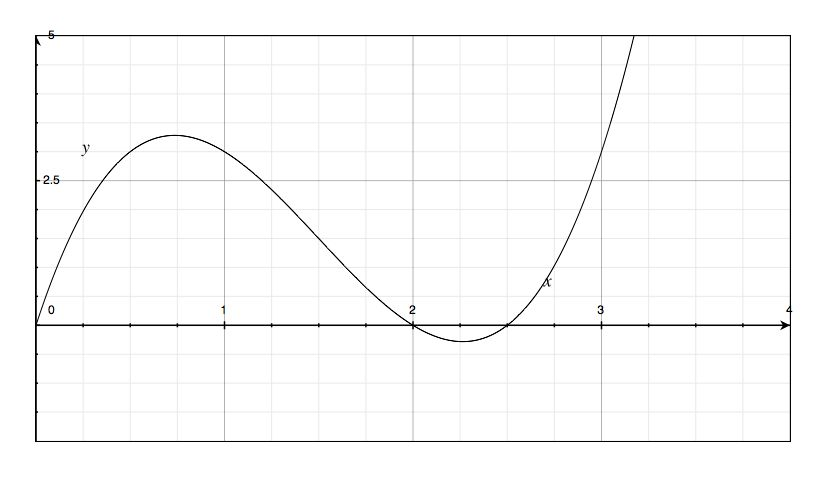
\includegraphics[width=\linewidth]{images/Math140S13wksht5g1.jpg}
\end{image}%
 When is the velocity of the particle positive, and when is it negative?%
\textbf{\blocktitlefont Solution}.\hypertarget{g:solution:idm389855904832}{}\quad{}The velocity of the particle is positive when the function is increasing, so \(0 < t < .75 \) and \(t > 2.25\). The velocity of the particle is negative when the function is decreasing, so \(.75 < t < 2.25\).%
\end{divisionexercise}%
\begin{divisionexercise}{3}{}{}{g:exercise:idm389855903952}%
Compute the derivative at a point \(f'(1)\) of \(f(x)=-3x^2+7x-2\) using the limit definition of the derivative.%
\textbf{\blocktitlefont Solution}.\hypertarget{g:solution:idm389855925648}{}\quad{}%
\begin{equation*}
f'(1) = \lim_{h\to 0} \frac{f(1+h)-f(1)}{h} 
\end{equation*}
%
\begin{equation*}
= \lim_{h\to 0} \frac{-3(1+h)^2+7(1+h)-2-(2)}{h}
\end{equation*}
%
\begin{equation*}
= \lim_{h\to 0} \frac{-3-6h-3h^2+7+7h-4}{h}
\end{equation*}
%
\begin{equation*}
= \lim_{h\to 0} \frac{-3h^2+h}{h} 
\end{equation*}
%
\begin{equation*}
= \lim_{h\to 0} -3h+1
\end{equation*}
%
\begin{equation*}
= 1 
\end{equation*}
\end{divisionexercise}%
\end{worksheet-subsection}
\restoregeometry
\setlength{\qrsize}{9em}
\setlength{\previewwidth}{\linewidth}
\addtolength{\previewwidth}{-\qrsize}
\begin{tcbraster}[raster columns=2, raster column skip=1pt, raster halign=center, raster force size=false, raster left skip=0pt, raster right skip=0pt]%
\begin{tcolorbox}[previewstyle, width=\previewwidth]%
\includegraphics[width=0.80\linewidth,height=\qrsize,keepaspectratio]{images/video-10.jpg}%
\end{tcolorbox}%
\begin{tcolorbox}[qrstyle]%
{\hypersetup{urlcolor=black}\qrcode[height=\qrsize]{https://www.youtube.com/watch?v=aiu5PdTHcLk}}%
\end{tcolorbox}%
\begin{tcolorbox}[captionstyle]%
\small YouTube: \mono{https://www.youtube.com/watch?v=aiu5PdTHcLk}\end{tcolorbox}%
\end{tcbraster}%
\end{sectionptx}
%
%
\typeout{************************************************}
\typeout{Section 2.2 Section 2.3 - The Derivative Function}
\typeout{************************************************}
%
\begin{sectionptx}{Section 2.3 - The Derivative Function}{}{Section 2.3 - The Derivative Function}{}{}{x:section:section2_3}
\setlength{\qrsize}{9em}
\setlength{\previewwidth}{\linewidth}
\addtolength{\previewwidth}{-\qrsize}
\begin{tcbraster}[raster columns=2, raster column skip=1pt, raster halign=center, raster force size=false, raster left skip=0pt, raster right skip=0pt]%
\begin{tcolorbox}[previewstyle, width=\previewwidth]%
\includegraphics[width=0.80\linewidth,height=\qrsize,keepaspectratio]{images/video-11.jpg}%
\end{tcolorbox}%
\begin{tcolorbox}[qrstyle]%
{\hypersetup{urlcolor=black}\qrcode[height=\qrsize]{https://www.youtube.com/watch?v=msvxJte7V4Y}}%
\end{tcolorbox}%
\begin{tcolorbox}[captionstyle]%
\small YouTube: \mono{https://www.youtube.com/watch?v=msvxJte7V4Y}\end{tcolorbox}%
\end{tcbraster}%
%
%
\typeout{************************************************}
\typeout{Worksheet 2.2.1 Worksheet}
\typeout{************************************************}
%
\newgeometry{left=1.25cm, right=1.25cm, top=1.25cm, bottom=1.25cm}
\begin{worksheet-subsection}{Worksheet}{}{Worksheet}{}{}{g:worksheet:idm389855981168}
\begin{divisionexercise}{1}{}{}{g:exercise:idm389855985632}%
The function \(f(x)\) is represented by the graph below. Sketch a graph of \(f'(x)\) on the axes below. \begin{image}{0}{1}{0}%
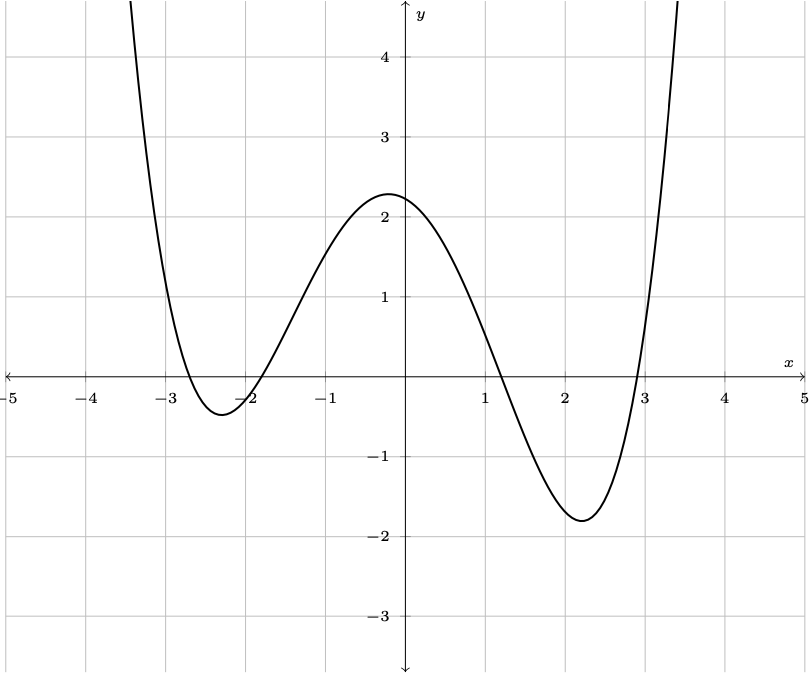
\includegraphics[width=\linewidth]{images/Math140WkshtDerivative2G1.png}
\end{image}%
%
\textbf{\blocktitlefont Solution}.\hypertarget{g:solution:idm389855999760}{}\quad{}\begin{image}{0}{1}{0}%
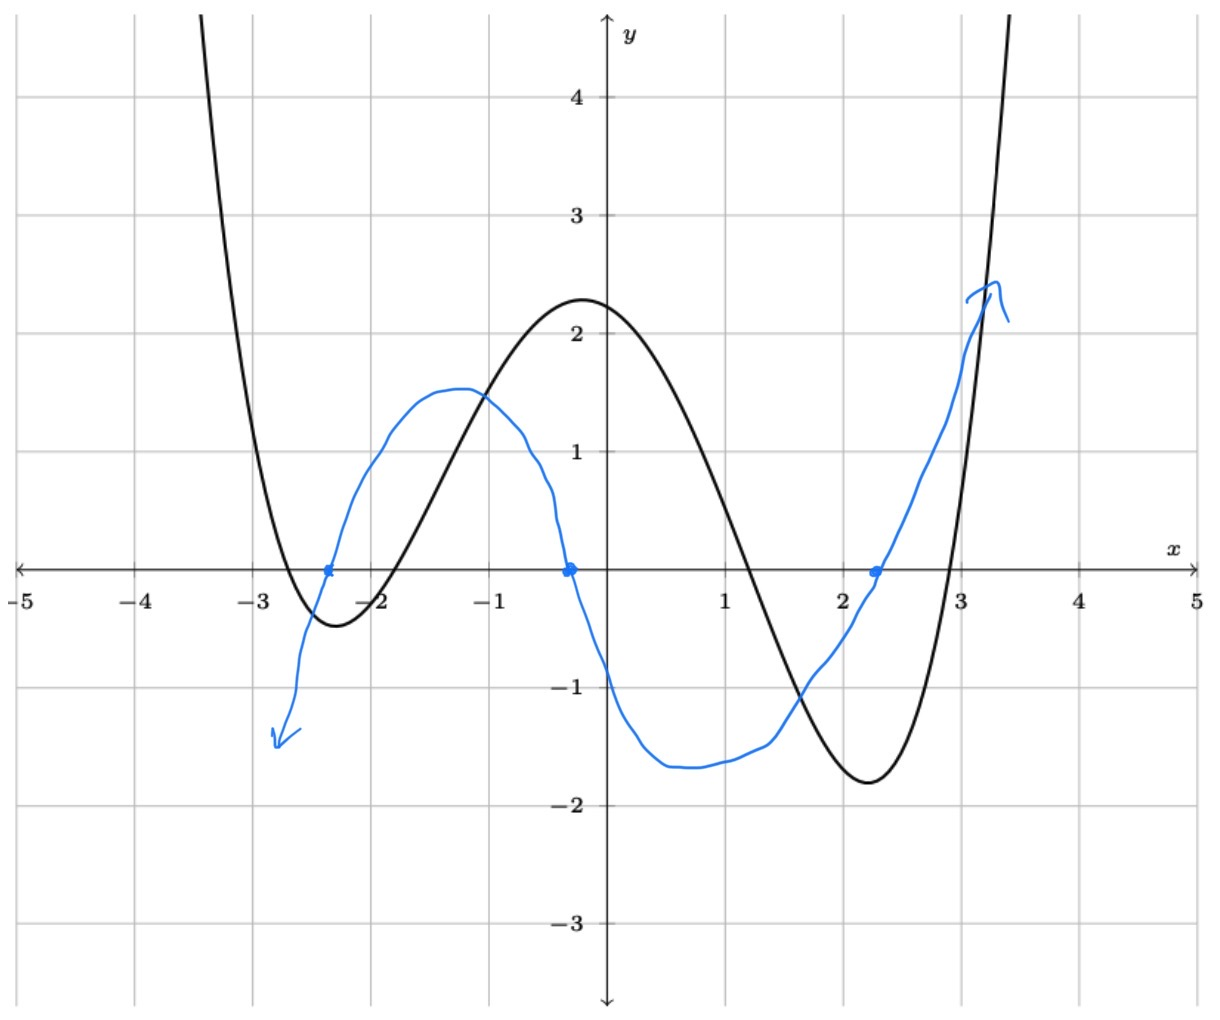
\includegraphics[width=\linewidth]{images/Math140WkshtDerivative2G2.JPG}
\end{image}%
\end{divisionexercise}%
\begin{divisionexercise}{2}{}{}{g:exercise:idm389837024448}%
If \(f(x) = x^2 - 4x+5\), compute \(f'(x)\) using the limit definition of the derivative.%
\textbf{\blocktitlefont Solution}.\hypertarget{g:solution:idm389776363712}{}\quad{}Using the limit definition we get%
\begin{align*}
f'(x) \amp = \lim_{h\to 0} \frac{f(x+h)-f(x)}{h} \\
\amp = \lim_{h\to 0} \frac{(x+h)^2-4(x+h)+5-(x^2-4x+5)}{h}\\
\amp = \lim_{h\to 0} \frac{x^2+2hx+h^2-4x-4h+5-x^2+4x-5}{h}\\
\amp = \lim_{h\to 0} \frac{2hx+h^2-4h}{h} \\
\amp = \lim_{h\to 0} \frac{h(2x+h-4)}{h}\\
\amp = \lim_{h\to 0} 2x+h-4 = 2x-4 
\end{align*}
\end{divisionexercise}%
\end{worksheet-subsection}
\restoregeometry
\setlength{\qrsize}{9em}
\setlength{\previewwidth}{\linewidth}
\addtolength{\previewwidth}{-\qrsize}
\begin{tcbraster}[raster columns=2, raster column skip=1pt, raster halign=center, raster force size=false, raster left skip=0pt, raster right skip=0pt]%
\begin{tcolorbox}[previewstyle, width=\previewwidth]%
\includegraphics[width=0.80\linewidth,height=\qrsize,keepaspectratio]{images/video-12.jpg}%
\end{tcolorbox}%
\begin{tcolorbox}[qrstyle]%
{\hypersetup{urlcolor=black}\qrcode[height=\qrsize]{https://www.youtube.com/watch?v=ZKFewXAYRrg}}%
\end{tcolorbox}%
\begin{tcolorbox}[captionstyle]%
\small YouTube: \mono{https://www.youtube.com/watch?v=ZKFewXAYRrg}\end{tcolorbox}%
\end{tcbraster}%
\end{sectionptx}
%
%
\typeout{************************************************}
\typeout{Section 2.3 Section 2.4 - Interpreting Derivatives}
\typeout{************************************************}
%
\begin{sectionptx}{Section 2.4 - Interpreting Derivatives}{}{Section 2.4 - Interpreting Derivatives}{}{}{x:section:section2_4}
\setlength{\qrsize}{9em}
\setlength{\previewwidth}{\linewidth}
\addtolength{\previewwidth}{-\qrsize}
\begin{tcbraster}[raster columns=2, raster column skip=1pt, raster halign=center, raster force size=false, raster left skip=0pt, raster right skip=0pt]%
\begin{tcolorbox}[previewstyle, width=\previewwidth]%
\includegraphics[width=0.80\linewidth,height=\qrsize,keepaspectratio]{images/video-13.jpg}%
\end{tcolorbox}%
\begin{tcolorbox}[qrstyle]%
{\hypersetup{urlcolor=black}\qrcode[height=\qrsize]{https://www.youtube.com/watch?v=bonR2NTmEeI}}%
\end{tcolorbox}%
\begin{tcolorbox}[captionstyle]%
\small YouTube: \mono{https://www.youtube.com/watch?v=bonR2NTmEeI}\end{tcolorbox}%
\end{tcbraster}%
%
%
\typeout{************************************************}
\typeout{Worksheet 2.3.1 Worksheet}
\typeout{************************************************}
%
\newgeometry{left=1.25cm, right=1.25cm, top=1.25cm, bottom=1.25cm}
\begin{worksheet-subsection}{Worksheet}{}{Worksheet}{}{}{g:worksheet:idm389776392912}
\begin{divisionexercise}{1}{}{}{g:exercise:idm389776393840}%
On a hot summer day, Bob takes a carton of ice cream out of a 10\(^\circ\)F freezer and forgets about it. Suppose room temperature is \(75^\circ\)F.%
%
\begin{enumerate}[label=(\alph*)]
\item{}Sketch a graph of temperature \(f(t)\) of the ice cream as a function of time, where \(t\) is time in hours.%
\par
\begin{image}{0}{1}{0}%
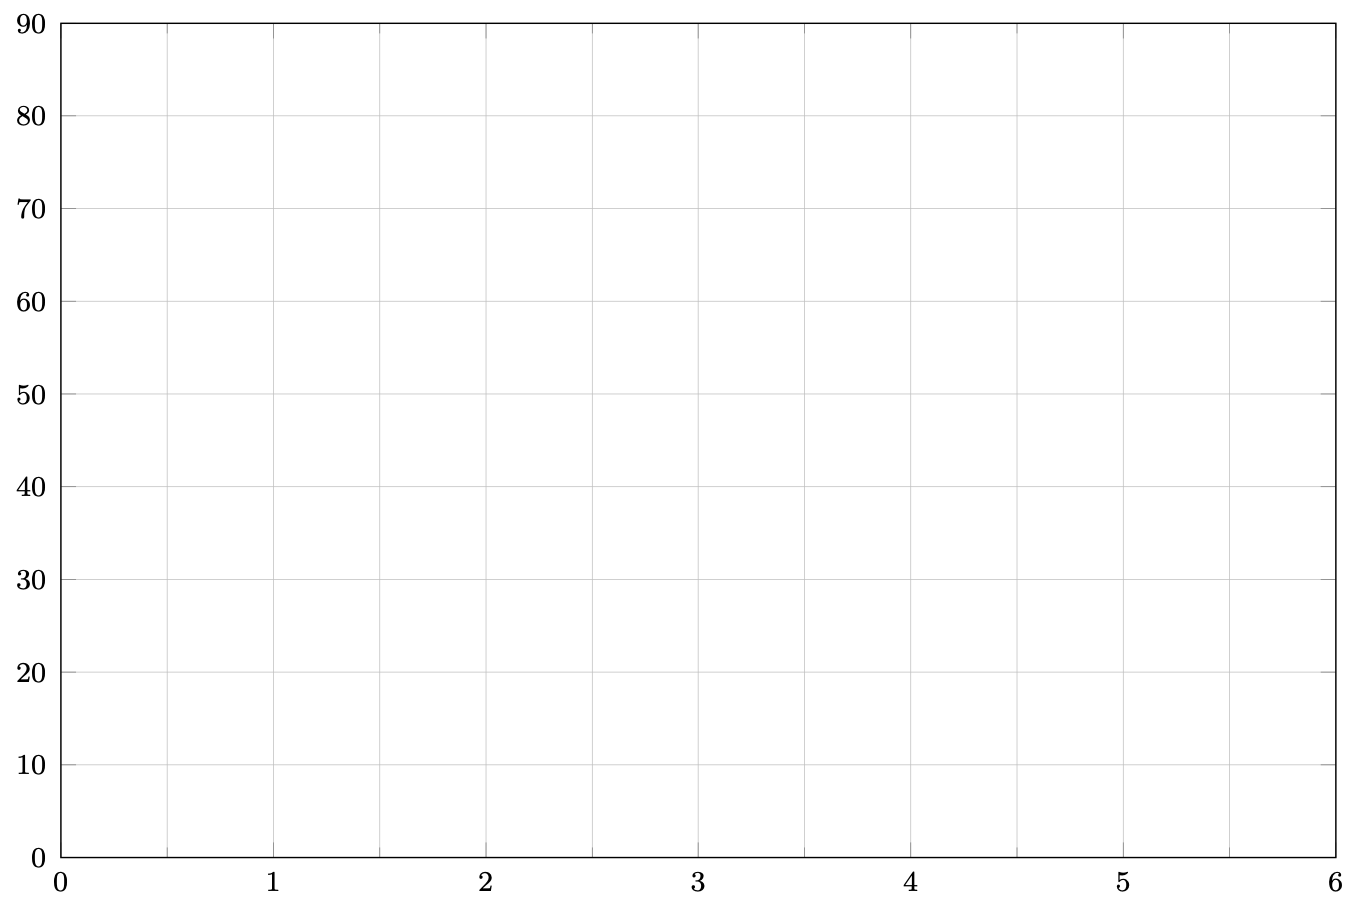
\includegraphics[width=\linewidth]{images/Math140WkshtInterpretingDerivativesG1.png}
\end{image}%
%
\item{}What are the units of \(f'(t)\)?%
\item{}Is the derivative positive or negative?%
\item{}Interpret the statement \(f'(4)=3\) in the context of the problem.%
\end{enumerate}
\textbf{\blocktitlefont Solution}.\hypertarget{g:solution:idm389776434304}{}\quad{}%
\begin{enumerate}[label=(\alph*)]
\item{}\begin{image}{0}{1}{0}%
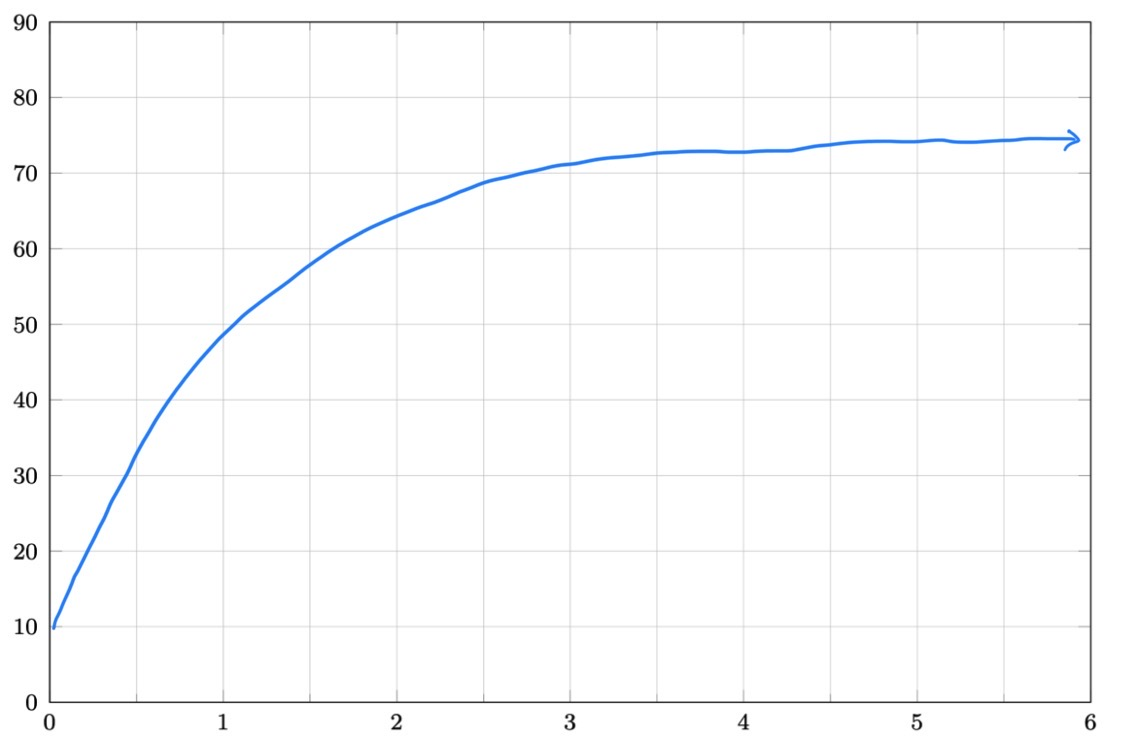
\includegraphics[width=\linewidth]{images/Math140WkshtInterpretingDerivativesG2.JPG}
\end{image}%
%
\item{}The units are \(^\circ\)F per hour (always output per input)%
\item{}The derivative is positive as the temperature is increasing%
\item{}After 4 hours, the temperature of the ice cream is increasing at a rate of 3\(^\circ\)F per hour.%
\end{enumerate}
\end{divisionexercise}%
\end{worksheet-subsection}
\restoregeometry
\setlength{\qrsize}{9em}
\setlength{\previewwidth}{\linewidth}
\addtolength{\previewwidth}{-\qrsize}
\begin{tcbraster}[raster columns=2, raster column skip=1pt, raster halign=center, raster force size=false, raster left skip=0pt, raster right skip=0pt]%
\begin{tcolorbox}[previewstyle, width=\previewwidth]%
\includegraphics[width=0.80\linewidth,height=\qrsize,keepaspectratio]{images/video-14.jpg}%
\end{tcolorbox}%
\begin{tcolorbox}[qrstyle]%
{\hypersetup{urlcolor=black}\qrcode[height=\qrsize]{https://www.youtube.com/watch?v=N4Dot_5pq7U}}%
\end{tcolorbox}%
\begin{tcolorbox}[captionstyle]%
\small YouTube: \mono{https://www.youtube.com/watch?v=N4Dot\_5pq7U}\end{tcolorbox}%
\end{tcbraster}%
\end{sectionptx}
%
%
\typeout{************************************************}
\typeout{Section 2.4 Section 2.5 - The Second Derivative}
\typeout{************************************************}
%
\begin{sectionptx}{Section 2.5 - The Second Derivative}{}{Section 2.5 - The Second Derivative}{}{}{x:section:section2_5}
\setlength{\qrsize}{9em}
\setlength{\previewwidth}{\linewidth}
\addtolength{\previewwidth}{-\qrsize}
\begin{tcbraster}[raster columns=2, raster column skip=1pt, raster halign=center, raster force size=false, raster left skip=0pt, raster right skip=0pt]%
\begin{tcolorbox}[previewstyle, width=\previewwidth]%
\includegraphics[width=0.80\linewidth,height=\qrsize,keepaspectratio]{images/video-15.jpg}%
\end{tcolorbox}%
\begin{tcolorbox}[qrstyle]%
{\hypersetup{urlcolor=black}\qrcode[height=\qrsize]{https://www.youtube.com/watch?v=4aLT6XeV9Gc}}%
\end{tcolorbox}%
\begin{tcolorbox}[captionstyle]%
\small YouTube: \mono{https://www.youtube.com/watch?v=4aLT6XeV9Gc}\end{tcolorbox}%
\end{tcbraster}%
%
%
\typeout{************************************************}
\typeout{Worksheet 2.4.1 Worksheet}
\typeout{************************************************}
%
\newgeometry{left=1.25cm, right=1.25cm, top=1.25cm, bottom=1.25cm}
\begin{worksheet-subsection}{Worksheet}{}{Worksheet}{}{}{g:worksheet:idm389776468672}
\begin{divisionexercise}{1}{}{}{g:exercise:idm389776469712}%
The table below gives the position \(s\) in feet of my car \(t\) seconds after I start merging onto the interstate.%
\begin{equation*}
\begin{array}{| l | l | l | l | l | l | l |}
\hline \text{Time } (t) & 0 & 2 & 4 & 6 & 8 & 10\\
\hline \text{Position} (s) & 0 & 20 & 52 & 90 & 132 & 200 \\
\hline
\end{array} 
\end{equation*}
%
%
\begin{enumerate}[label=(\alph*)]
\item{}Estimate \(\displaystyle \frac{ds}{dt}\) for the time intervals below%
\begin{equation*}
\begin{array}{| p{2.5cm} | p{2cm} | p{2cm} | p{2cm} | p{2cm} | p{2cm} |}
\hline \text{Time Interval} & 0-2 & 2-4 & 4-6 & 6-8 & 8-10\\
\hline \frac{ds}{dt} &  &  &  &  &  \\
\hline
\end{array} 
\end{equation*}
%
\item{}What can we say about \(\displaystyle \frac{d^2 s}{dt^2}\) over this period of time%
\end{enumerate}
\textbf{\blocktitlefont Solution}.\hypertarget{g:solution:idm389776470128}{}\quad{}%
\begin{enumerate}[label=(\alph*)]
\item{}We can estimate \(\displaystyle \frac{ds}{dt}\) for the time intervals below using the average rate of change.%
\begin{equation*}
\begin{array}{| p{2.5cm} | p{2cm} | p{2cm} | p{2cm} | p{2cm} | p{2cm} |}
\hline \text{Time Interval} & 0-2 & 2-4 & 4-6 & 6-8 & 8-10\\
\hline \frac{ds}{dt} &  \frac{20-0}{2-0} = 10 & 16  & 19 & 21 & 34 \\
\hline
\end{array} 
\end{equation*}
%
\item{}The second derivative is positive as it appears that the derivative is increasing.%
\end{enumerate}
\end{divisionexercise}%
\begin{divisionexercise}{2}{}{}{g:exercise:idm389776518272}%
Compute the second derivative of%
\begin{equation*}
f(x) = 3x^2+7x+1 . 
\end{equation*}
%
\textbf{\blocktitlefont Solution}.\hypertarget{g:solution:idm389776522304}{}\quad{}Using the limit of the difference quotient, we get%
\begin{align*}
f'(x)  \amp = \lim_{h\to 0} \frac{f(x+h)-f(x)}{h} \\
\amp = \lim_{h\to 0} \frac{3x^2+6xh+3h^2+7x+7h+1 - (3x^2+7x+1)}{h} \\
\amp = \lim_{h\to 0} \frac{6xh+3h^2+7h}{h} \\
\amp = \lim_{h\to 0} 6x+3h+7\\
\amp = 6x+7
\end{align*}
To compute the second derivative, we take the derivative of \(f'(x)\) as above. Since it is linear, the derivative is the slope which is 6 in this case.%
\end{divisionexercise}%
\begin{divisionexercise}{3}{}{}{g:exercise:idm389776540224}%
\footnotemark{}The following graph is the graph of the position function of a particle traveling in a straight line.%
\par
\begin{image}{0}{1}{0}%
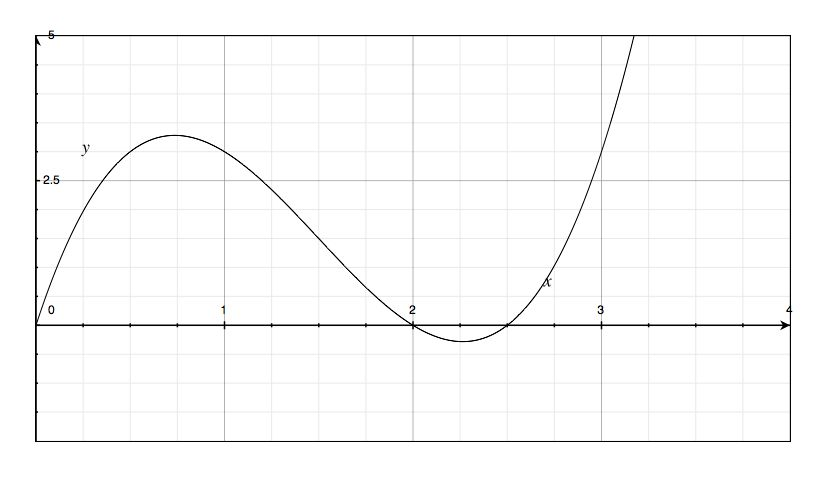
\includegraphics[width=\linewidth]{images/Math140S13wksht5g1.jpg}
\end{image}%
%
%
\begin{enumerate}[label=(\alph*)]
\item{}When is the acceleration of the particle positive, and when is it negative?%
\item{}When is the acceleration zero?%
\end{enumerate}
\textbf{\blocktitlefont Solution}.\hypertarget{g:solution:idm389776550656}{}\quad{}%
\begin{enumerate}[label=(\alph*)]
\item{}The acceleration of the particle is positive when the graph is concave up. This looks to be \(x>1.5\). The acceleration is negative when the graph is concave down. This looks to be \(x< 1.5\).%
\item{}The acceleration appears to be zero at 1.5%
\end{enumerate}
\end{divisionexercise}%
\footnotetext[1]{Similar to Example 5 in Section 2.5\label{g:fn:idm389776541312}}%
\end{worksheet-subsection}
\restoregeometry
\setlength{\qrsize}{9em}
\setlength{\previewwidth}{\linewidth}
\addtolength{\previewwidth}{-\qrsize}
\begin{tcbraster}[raster columns=2, raster column skip=1pt, raster halign=center, raster force size=false, raster left skip=0pt, raster right skip=0pt]%
\begin{tcolorbox}[previewstyle, width=\previewwidth]%
\includegraphics[width=0.80\linewidth,height=\qrsize,keepaspectratio]{images/video-16.jpg}%
\end{tcolorbox}%
\begin{tcolorbox}[qrstyle]%
{\hypersetup{urlcolor=black}\qrcode[height=\qrsize]{https://www.youtube.com/watch?v=6KvGtxdqehs}}%
\end{tcolorbox}%
\begin{tcolorbox}[captionstyle]%
\small YouTube: \mono{https://www.youtube.com/watch?v=6KvGtxdqehs}\end{tcolorbox}%
\end{tcbraster}%
\end{sectionptx}
%
%
\typeout{************************************************}
\typeout{Section 2.5 Section 2.6 - Differentiability}
\typeout{************************************************}
%
\begin{sectionptx}{Section 2.6 - Differentiability}{}{Section 2.6 - Differentiability}{}{}{x:section:section2_6}
\setlength{\qrsize}{9em}
\setlength{\previewwidth}{\linewidth}
\addtolength{\previewwidth}{-\qrsize}
\begin{tcbraster}[raster columns=2, raster column skip=1pt, raster halign=center, raster force size=false, raster left skip=0pt, raster right skip=0pt]%
\begin{tcolorbox}[previewstyle, width=\previewwidth]%
\includegraphics[width=0.80\linewidth,height=\qrsize,keepaspectratio]{images/video-17.jpg}%
\end{tcolorbox}%
\begin{tcolorbox}[qrstyle]%
{\hypersetup{urlcolor=black}\qrcode[height=\qrsize]{https://www.youtube.com/watch?v=XMQqubhCCOs}}%
\end{tcolorbox}%
\begin{tcolorbox}[captionstyle]%
\small YouTube: \mono{https://www.youtube.com/watch?v=XMQqubhCCOs}\end{tcolorbox}%
\end{tcbraster}%
\end{sectionptx}
\end{chapterptx}
%
%
\typeout{************************************************}
\typeout{Chapter 3 Week 3 - Derivative Rules}
\typeout{************************************************}
%
\begin{chapterptx}{Week 3 - Derivative Rules}{}{Week 3 - Derivative Rules}{}{}{x:chapter:week3}
%
%
\typeout{************************************************}
\typeout{Section 3.1 Section 3.1 - Powers \& Polynomials}
\typeout{************************************************}
%
\begin{sectionptx}{Section 3.1 - Powers \& Polynomials}{}{Section 3.1 - Powers \& Polynomials}{}{}{x:section:section3_1}
\setlength{\qrsize}{9em}
\setlength{\previewwidth}{\linewidth}
\addtolength{\previewwidth}{-\qrsize}
\begin{tcbraster}[raster columns=2, raster column skip=1pt, raster halign=center, raster force size=false, raster left skip=0pt, raster right skip=0pt]%
\begin{tcolorbox}[previewstyle, width=\previewwidth]%
\includegraphics[width=0.80\linewidth,height=\qrsize,keepaspectratio]{images/video-18.jpg}%
\end{tcolorbox}%
\begin{tcolorbox}[qrstyle]%
{\hypersetup{urlcolor=black}\qrcode[height=\qrsize]{https://www.youtube.com/watch?v=2MYJKakPOBs}}%
\end{tcolorbox}%
\begin{tcolorbox}[captionstyle]%
\small YouTube: \mono{https://www.youtube.com/watch?v=2MYJKakPOBs}\end{tcolorbox}%
\end{tcbraster}%
%
%
\typeout{************************************************}
\typeout{Worksheet 3.1.1 Worksheet}
\typeout{************************************************}
%
\newgeometry{left=1.25cm, right=1.25cm, top=1.25cm, bottom=1.25cm}
\begin{worksheet-subsection}{Worksheet}{}{Worksheet}{}{}{g:worksheet:idm389776576096}
\begin{divisionexercise}{1}{}{}{g:exercise:idm389776577824}%
Compute the derivatives of the following functions%
%
\begin{enumerate}[label=(\alph*)]
\item{}\(\displaystyle f(t) = 3t^2-4t+1\)%
\item{}\(\displaystyle g(x) = 17x^{3/2} - 5x^{1/2}\)%
\item{}\(\displaystyle h(t) = 3t^2 + \frac{12}{\sqrt t} - \frac{1}{t^2}\)%
\item{}\(\displaystyle k(x) = \frac{\sqrt x (1+x)}{x^2}\)%
\end{enumerate}
\textbf{\blocktitlefont Solution}.\hypertarget{g:solution:idm389856018832}{}\quad{}%
\begin{enumerate}[label=(\alph*)]
\item{}\(\displaystyle f'(t) = 6t-4 \)%
\item{}\(\displaystyle g(x) = \left(\frac{51}{2}\right)x^{1/2} - \left( \frac 52 \right) x^{-1/2}\)%
\item{}\(\displaystyle h(t) = 6t -6t^{-3/2} +2t^{-3}\)%
\item{}\(\displaystyle k(x) = -\frac 32 x^{-5/2} - \frac 12 x^{-3/2}\)%
\end{enumerate}
\end{divisionexercise}%
\begin{divisionexercise}{2}{}{}{g:exercise:idm389856030976}%
A raindrop falls from a cloud with height (in meters) given as a function of time by%
\begin{equation*}
h=1000-4.9t^2.
\end{equation*}
Find the velocity and acceleration at time \(t\).%
\textbf{\blocktitlefont Solution}.\hypertarget{g:solution:idm389856035120}{}\quad{}The velocity is the derivative%
\begin{equation*}
\frac{dh}{dt} = -9.8 t \text{ m}/\text{sec}
\end{equation*}
and the acceleration is the second derivative%
\begin{equation*}
\frac{d^2h}{dt^2} = -9.8 \text{ m}/\text{sec}^2
\end{equation*}
%
\end{divisionexercise}%
\end{worksheet-subsection}
\restoregeometry
\setlength{\qrsize}{9em}
\setlength{\previewwidth}{\linewidth}
\addtolength{\previewwidth}{-\qrsize}
\begin{tcbraster}[raster columns=2, raster column skip=1pt, raster halign=center, raster force size=false, raster left skip=0pt, raster right skip=0pt]%
\begin{tcolorbox}[previewstyle, width=\previewwidth]%
\includegraphics[width=0.80\linewidth,height=\qrsize,keepaspectratio]{images/video-19.jpg}%
\end{tcolorbox}%
\begin{tcolorbox}[qrstyle]%
{\hypersetup{urlcolor=black}\qrcode[height=\qrsize]{https://www.youtube.com/watch?v=v6xWL_qKdt0}}%
\end{tcolorbox}%
\begin{tcolorbox}[captionstyle]%
\small YouTube: \mono{https://www.youtube.com/watch?v=v6xWL\_qKdt0}\end{tcolorbox}%
\end{tcbraster}%
\end{sectionptx}
%
%
\typeout{************************************************}
\typeout{Section 3.2 Section 3.2 - The Exponential Function}
\typeout{************************************************}
%
\begin{sectionptx}{Section 3.2 - The Exponential Function}{}{Section 3.2 - The Exponential Function}{}{}{x:section:section3_2}
\setlength{\qrsize}{9em}
\setlength{\previewwidth}{\linewidth}
\addtolength{\previewwidth}{-\qrsize}
\begin{tcbraster}[raster columns=2, raster column skip=1pt, raster halign=center, raster force size=false, raster left skip=0pt, raster right skip=0pt]%
\begin{tcolorbox}[previewstyle, width=\previewwidth]%
\includegraphics[width=0.80\linewidth,height=\qrsize,keepaspectratio]{images/video-20.jpg}%
\end{tcolorbox}%
\begin{tcolorbox}[qrstyle]%
{\hypersetup{urlcolor=black}\qrcode[height=\qrsize]{https://www.youtube.com/watch?v=F4dke9WKQXM}}%
\end{tcolorbox}%
\begin{tcolorbox}[captionstyle]%
\small YouTube: \mono{https://www.youtube.com/watch?v=F4dke9WKQXM}\end{tcolorbox}%
\end{tcbraster}%
%
%
\typeout{************************************************}
\typeout{Worksheet 3.2.1 Worksheet}
\typeout{************************************************}
%
\newgeometry{left=1.25cm, right=1.25cm, top=1.25cm, bottom=1.25cm}
\begin{worksheet-subsection}{Worksheet}{}{Worksheet}{}{}{g:worksheet:idm389856050880}
\begin{divisionexercise}{1}{}{}{g:exercise:idm389856054400}%
Compute the derivatives of the following functions%
%
\begin{enumerate}[label=(\alph*)]
\item{}\(\displaystyle f(t) = 5\cdot 2^t\)%
\item{}\(\displaystyle g(x) = e^{3x}\)%
\item{}\(\displaystyle h(t) = e^{t+3}\)%
\item{}\(\displaystyle k(x) = \pi^{\pi}+\pi^x+x^{\pi}\)%
\end{enumerate}
\textbf{\blocktitlefont Solution}.\hypertarget{g:solution:idm389856063296}{}\quad{}%
\begin{enumerate}[label=(\alph*)]
\item{}\(\displaystyle f'(t) = 5\cdot 2^t \ln(2)\)%
\item{}\(\displaystyle g'(x) = e^{3x}\cdot 3\)%
\item{}\(\displaystyle h'(t) = e^{t+3}\)%
\item{}\(\displaystyle k'(x) = 0+\pi^x\ln(\pi)+\pi x^{\pi-1}\)%
\end{enumerate}
\end{divisionexercise}%
\end{worksheet-subsection}
\restoregeometry
\setlength{\qrsize}{9em}
\setlength{\previewwidth}{\linewidth}
\addtolength{\previewwidth}{-\qrsize}
\begin{tcbraster}[raster columns=2, raster column skip=1pt, raster halign=center, raster force size=false, raster left skip=0pt, raster right skip=0pt]%
\begin{tcolorbox}[previewstyle, width=\previewwidth]%
\includegraphics[width=0.80\linewidth,height=\qrsize,keepaspectratio]{images/video-21.jpg}%
\end{tcolorbox}%
\begin{tcolorbox}[qrstyle]%
{\hypersetup{urlcolor=black}\qrcode[height=\qrsize]{https://www.youtube.com/watch?v=4pnJa1cmNjI}}%
\end{tcolorbox}%
\begin{tcolorbox}[captionstyle]%
\small YouTube: \mono{https://www.youtube.com/watch?v=4pnJa1cmNjI}\end{tcolorbox}%
\end{tcbraster}%
\end{sectionptx}
%
%
\typeout{************************************************}
\typeout{Section 3.3 Section 3.3 - Product \& Quotient Rules}
\typeout{************************************************}
%
\begin{sectionptx}{Section 3.3 - Product \& Quotient Rules}{}{Section 3.3 - Product \& Quotient Rules}{}{}{x:section:section3_3}
\setlength{\qrsize}{9em}
\setlength{\previewwidth}{\linewidth}
\addtolength{\previewwidth}{-\qrsize}
\begin{tcbraster}[raster columns=2, raster column skip=1pt, raster halign=center, raster force size=false, raster left skip=0pt, raster right skip=0pt]%
\begin{tcolorbox}[previewstyle, width=\previewwidth]%
\includegraphics[width=0.80\linewidth,height=\qrsize,keepaspectratio]{images/video-22.jpg}%
\end{tcolorbox}%
\begin{tcolorbox}[qrstyle]%
{\hypersetup{urlcolor=black}\qrcode[height=\qrsize]{https://www.youtube.com/watch?v=h6uYz4T2xtk}}%
\end{tcolorbox}%
\begin{tcolorbox}[captionstyle]%
\small YouTube: \mono{https://www.youtube.com/watch?v=h6uYz4T2xtk}\end{tcolorbox}%
\end{tcbraster}%
%
%
\typeout{************************************************}
\typeout{Worksheet 3.3.1 Worksheet}
\typeout{************************************************}
%
\newgeometry{left=1.25cm, right=1.25cm, top=1.25cm, bottom=1.25cm}
\begin{worksheet-subsection}{Worksheet}{}{Worksheet}{}{}{g:worksheet:idm389856086768}
\begin{divisionexercise}{1}{}{}{g:exercise:idm389856087776}%
Compute the derivatives of the following functions:%
%
\begin{enumerate}[label=(\alph*)]
\item{}\(\displaystyle f(x) = x^3 3^x\)%
\item{}\(\displaystyle g(x) = \frac{x^2 + e^x}{x^3}\)%
\item{}\(\displaystyle h(x) = \frac{x^2+7}{x^2-7}\)%
\item{}\(\displaystyle k(x) = e^{x+5}(x^2+3x)\)%
\end{enumerate}
\textbf{\blocktitlefont Solution}.\hypertarget{g:solution:idm389856108992}{}\quad{}%
\begin{enumerate}[label=(\alph*)]
\item{}\(\displaystyle f'(x) = x^3 3^x\ln(3)+3^x(3x^2)\)%
\item{}\(\displaystyle g'(x) = \frac{(x^3)(2x+e^x)-(x^2 + e^x)(3x^2)}{(x^3)^2}\)%
\item{}\(\displaystyle h'(x) = \frac{(x^2-7)(2x)-(x^2+7)(2x)}{(x^2-7)^2}\)%
\item{}\(\displaystyle k(x) = e^{x+5}(2x+3)+(x^2+3x)e^{x+5}\)%
\end{enumerate}
\end{divisionexercise}%
\end{worksheet-subsection}
\restoregeometry
\setlength{\qrsize}{9em}
\setlength{\previewwidth}{\linewidth}
\addtolength{\previewwidth}{-\qrsize}
\begin{tcbraster}[raster columns=2, raster column skip=1pt, raster halign=center, raster force size=false, raster left skip=0pt, raster right skip=0pt]%
\begin{tcolorbox}[previewstyle, width=\previewwidth]%
\includegraphics[width=0.80\linewidth,height=\qrsize,keepaspectratio]{images/video-23.jpg}%
\end{tcolorbox}%
\begin{tcolorbox}[qrstyle]%
{\hypersetup{urlcolor=black}\qrcode[height=\qrsize]{https://www.youtube.com/watch?v=aKmx4mJ-b2Q}}%
\end{tcolorbox}%
\begin{tcolorbox}[captionstyle]%
\small YouTube: \mono{https://www.youtube.com/watch?v=aKmx4mJ-b2Q}\end{tcolorbox}%
\end{tcbraster}%
\end{sectionptx}
%
%
\typeout{************************************************}
\typeout{Section 3.4 Section 3.4 - The Chain Rule}
\typeout{************************************************}
%
\begin{sectionptx}{Section 3.4 - The Chain Rule}{}{Section 3.4 - The Chain Rule}{}{}{x:section:section3_4}
\setlength{\qrsize}{9em}
\setlength{\previewwidth}{\linewidth}
\addtolength{\previewwidth}{-\qrsize}
\begin{tcbraster}[raster columns=2, raster column skip=1pt, raster halign=center, raster force size=false, raster left skip=0pt, raster right skip=0pt]%
\begin{tcolorbox}[previewstyle, width=\previewwidth]%
\includegraphics[width=0.80\linewidth,height=\qrsize,keepaspectratio]{images/video-24.jpg}%
\end{tcolorbox}%
\begin{tcolorbox}[qrstyle]%
{\hypersetup{urlcolor=black}\qrcode[height=\qrsize]{https://www.youtube.com/watch?v=PGwkvz2tYyY}}%
\end{tcolorbox}%
\begin{tcolorbox}[captionstyle]%
\small YouTube: \mono{https://www.youtube.com/watch?v=PGwkvz2tYyY}\end{tcolorbox}%
\end{tcbraster}%
%
%
\typeout{************************************************}
\typeout{Worksheet 3.4.1 Worksheet}
\typeout{************************************************}
%
\newgeometry{left=1.25cm, right=1.25cm, top=1.25cm, bottom=1.25cm}
\begin{worksheet-subsection}{Worksheet}{}{Worksheet}{}{}{g:worksheet:idm389856127664}
\begin{divisionexercise}{1}{}{}{g:exercise:idm389856129104}%
Compute the derivatives of the following functions using the chain rule:%
%
\begin{enumerate}[label=(\alph*)]
\item{}\(\displaystyle k(x) = e^{x+1}\)%
\item{}\(\displaystyle f(x) = \sqrt{e^x +1}\)%
\item{}\(\displaystyle g(t) = (\sqrt{t} + 1)^{100}\)%
\item{}\(\displaystyle h(x) = \sqrt{ \frac{x^2+9}{x+3}}\)%
\item{}\(\displaystyle k(x) = e^{(x^2)}\)%
\end{enumerate}
\textbf{\blocktitlefont Solution}.\hypertarget{g:solution:idm389856139696}{}\quad{}%
\begin{enumerate}[label=(\alph*)]
\item{}\(\displaystyle k'(x) = e^{x+1}\)%
\item{}\(\displaystyle f'(x) = \frac 12 (e^x +1)^{-1/2}(e^x)\)%
\item{}\(\displaystyle g(t) = 100(\sqrt{t} + 1)^{99}\left( \frac 12 t^{-1/2} \right)\)%
\item{}\(\displaystyle h(x) = \frac 12 \left( \frac{x^2+9}{x+3} \right) ^{-1/2} \left( \frac{(x+3)(2x)-(x^2+9)(1)}{(x+3)^2} \right)\)%
\item{}\(\displaystyle k(x) = e^{(x^2)} (2x)\)%
\end{enumerate}
\end{divisionexercise}%
\end{worksheet-subsection}
\restoregeometry
\setlength{\qrsize}{9em}
\setlength{\previewwidth}{\linewidth}
\addtolength{\previewwidth}{-\qrsize}
\begin{tcbraster}[raster columns=2, raster column skip=1pt, raster halign=center, raster force size=false, raster left skip=0pt, raster right skip=0pt]%
\begin{tcolorbox}[previewstyle, width=\previewwidth]%
\includegraphics[width=0.80\linewidth,height=\qrsize,keepaspectratio]{images/video-25.jpg}%
\end{tcolorbox}%
\begin{tcolorbox}[qrstyle]%
{\hypersetup{urlcolor=black}\qrcode[height=\qrsize]{https://www.youtube.com/watch?v=ksltkNMjLLg}}%
\end{tcolorbox}%
\begin{tcolorbox}[captionstyle]%
\small YouTube: \mono{https://www.youtube.com/watch?v=ksltkNMjLLg}\end{tcolorbox}%
\end{tcbraster}%
\end{sectionptx}
\end{chapterptx}
%
%
\typeout{************************************************}
\typeout{Chapter 4 Week 4 - More Derivative Rules}
\typeout{************************************************}
%
\begin{chapterptx}{Week 4 - More Derivative Rules}{}{Week 4 - More Derivative Rules}{}{}{x:chapter:week4}
%
%
\typeout{************************************************}
\typeout{Section 4.1 Section 3.5 - Trigonometric Functions}
\typeout{************************************************}
%
\begin{sectionptx}{Section 3.5 - Trigonometric Functions}{}{Section 3.5 - Trigonometric Functions}{}{}{x:section:section3_5}
\setlength{\qrsize}{9em}
\setlength{\previewwidth}{\linewidth}
\addtolength{\previewwidth}{-\qrsize}
\begin{tcbraster}[raster columns=2, raster column skip=1pt, raster halign=center, raster force size=false, raster left skip=0pt, raster right skip=0pt]%
\begin{tcolorbox}[previewstyle, width=\previewwidth]%
\includegraphics[width=0.80\linewidth,height=\qrsize,keepaspectratio]{images/video-26.jpg}%
\end{tcolorbox}%
\begin{tcolorbox}[qrstyle]%
{\hypersetup{urlcolor=black}\qrcode[height=\qrsize]{https://www.youtube.com/watch?v=EtJwmbpXxVI}}%
\end{tcolorbox}%
\begin{tcolorbox}[captionstyle]%
\small YouTube: \mono{https://www.youtube.com/watch?v=EtJwmbpXxVI}\end{tcolorbox}%
\end{tcbraster}%
%
%
\typeout{************************************************}
\typeout{Worksheet 4.1.1 Worksheet}
\typeout{************************************************}
%
\newgeometry{left=1.25cm, right=1.25cm, top=1.25cm, bottom=1.25cm}
\begin{worksheet-subsection}{Worksheet}{}{Worksheet}{}{}{g:worksheet:idm389856157952}
\begin{divisionexercise}{1}{}{}{g:exercise:idm389856159280}%
So we know that%
\begin{equation*}
\frac{d}{dx} ( \sin x ) = \cos x \hspace{.2in} \text{ and } \hspace{.2in} \frac{d}{dx} (\cos x) = - \sin x 
\end{equation*}
and we know that%
\begin{equation*}
\tan x = \frac{\sin x}{\cos x} . 
\end{equation*}
Compute the derivative of \(\tan x\).%
\textbf{\blocktitlefont Solution}.\hypertarget{g:solution:idm389856168608}{}\quad{}Using the quotient rule, we get%
\begin{equation*}
\frac{d}{dx}\left( \tan x \right) = \frac{d}{dx}\left( \frac{\sin x}{\cos x} \right) = \frac{\cos(x)\cos(x)-\sin(x)(-\sin(x))}{(\cos(x))^2}
\end{equation*}
%
\begin{equation*}
= \frac{(\cos(x))^2+(\sin(x))^2}{(\cos(x))^2} = \frac{1}{(\cos(x))^2} 
\end{equation*}
The last equality comes from the Pythagorean Identity.%
\end{divisionexercise}%
\begin{divisionexercise}{2}{}{}{g:exercise:idm389856176976}%
\footnotemark{} The voltage, \(V\), in volts, in an electrical outlet is given as a function of time, \(t\), in second by the function%
\begin{equation*}
V = 156 \cos(120 \pi t) 
\end{equation*}
%
%
\begin{enumerate}[label=(\alph*)]
\item{}Give an expression for the rate of change of voltage with respect to time.%
\item{}What is the maximum rate of change?%
\end{enumerate}
\textbf{\blocktitlefont Solution}.\hypertarget{g:solution:idm389856178064}{}\quad{}%
\begin{enumerate}[label=(\alph*)]
\item{}\(\displaystyle \frac{dV}{dt} = 156(-\sin(120\pi t))(120\pi)\)%
\item{}The maximum that \(-\sin(120 \pi t)\) can be is 1 as -1 is the minimum of the sine function. Thus, the maximum of the derivative here is \(156\cdot 120\pi\).%
\end{enumerate}
\end{divisionexercise}%
\footnotetext[1]{From problem 62 in section 3.5\label{g:fn:idm389856178320}}%
\begin{divisionexercise}{3}{}{}{g:exercise:idm389856200224}%
Compute the following derivatives:%
%
\begin{enumerate}[label=(\alph*)]
\item{}\(\displaystyle \displaystyle \frac{d}{dx} (\sin(x^2))\)%
\item{}\(\displaystyle \displaystyle\frac{d}{dx} \left( \frac{3\cos(x)}{x^2-7}\right)\)%
\item{}\(\displaystyle\frac{d}{dx} \left( \frac{\cos(x)}{\sin(x)} \right)\)  (p.s. Do you know a name for this function?)%
\item{}\(\displaystyle \displaystyle\frac{d}{dx} \left( e^{\sin(x)} \right)\)%
\end{enumerate}
\textbf{\blocktitlefont Solution}.\hypertarget{g:solution:idm389856209152}{}\quad{}%
\begin{enumerate}[label=(\alph*)]
\item{}\(\displaystyle \displaystyle \frac{d}{dx} (\sin(x^2))= \cos(x^2)\cdot (2x)\)%
\item{}\(\displaystyle \displaystyle\frac{d}{dx} \left( \frac{3\cos(x)}{x^2-7}\right)= \frac{(x^2-7)(3(-\sin(x)))-(3\cos(x))(2x)}{(x^2-7)^2}\)%
\item{}\(\displaystyle\frac{d}{dx} \left( \frac{\cos(x)}{\sin(x)} \right) = \frac{\sin(x)(-\sin(x))-(\cos(x))(\cos(x))}{(\sin(x))^2} = \frac{-1}{(\sin(x))^2} \) (the original function is cotangent)%
\item{}\(\displaystyle \displaystyle\frac{d}{dx} \left( e^{\sin(x)} \right) = e^{\sin(x)}\cos(x)\)%
\end{enumerate}
\end{divisionexercise}%
\end{worksheet-subsection}
\restoregeometry
\setlength{\qrsize}{9em}
\setlength{\previewwidth}{\linewidth}
\addtolength{\previewwidth}{-\qrsize}
\begin{tcbraster}[raster columns=2, raster column skip=1pt, raster halign=center, raster force size=false, raster left skip=0pt, raster right skip=0pt]%
\begin{tcolorbox}[previewstyle, width=\previewwidth]%
\includegraphics[width=0.80\linewidth,height=\qrsize,keepaspectratio]{images/video-27.jpg}%
\end{tcolorbox}%
\begin{tcolorbox}[qrstyle]%
{\hypersetup{urlcolor=black}\qrcode[height=\qrsize]{https://www.youtube.com/watch?v=5UFYu0TRcbA}}%
\end{tcolorbox}%
\begin{tcolorbox}[captionstyle]%
\small YouTube: \mono{https://www.youtube.com/watch?v=5UFYu0TRcbA}\end{tcolorbox}%
\end{tcbraster}%
\end{sectionptx}
%
%
\typeout{************************************************}
\typeout{Section 4.2 Section 3.6 - Inverse Functions}
\typeout{************************************************}
%
\begin{sectionptx}{Section 3.6 - Inverse Functions}{}{Section 3.6 - Inverse Functions}{}{}{x:section:section3_6}
\setlength{\qrsize}{9em}
\setlength{\previewwidth}{\linewidth}
\addtolength{\previewwidth}{-\qrsize}
\begin{tcbraster}[raster columns=2, raster column skip=1pt, raster halign=center, raster force size=false, raster left skip=0pt, raster right skip=0pt]%
\begin{tcolorbox}[previewstyle, width=\previewwidth]%
\includegraphics[width=0.80\linewidth,height=\qrsize,keepaspectratio]{images/video-28.jpg}%
\end{tcolorbox}%
\begin{tcolorbox}[qrstyle]%
{\hypersetup{urlcolor=black}\qrcode[height=\qrsize]{https://www.youtube.com/watch?v=H4Gp5Xlsh-E}}%
\end{tcolorbox}%
\begin{tcolorbox}[captionstyle]%
\small YouTube: \mono{https://www.youtube.com/watch?v=H4Gp5Xlsh-E}\end{tcolorbox}%
\end{tcbraster}%
%
%
\typeout{************************************************}
\typeout{Worksheet 4.2.1 Worksheet}
\typeout{************************************************}
%
\newgeometry{left=1.25cm, right=1.25cm, top=1.25cm, bottom=1.25cm}
\begin{worksheet-subsection}{Worksheet}{}{Worksheet}{}{}{g:worksheet:idm389856221952}
\begin{divisionexercise}{1}{}{}{g:exercise:idm389856222896}%
Compute the derivative of the following functions:%
%
\begin{enumerate}[label=(\alph*)]
\item{}\(\displaystyle f(x) = \ln(2^x+x^2)\)%
\item{}\(\displaystyle g(t) = \sqrt{\arcsin(t)}\)%
\item{}\(\displaystyle h(x) = \arctan(\ln(x))\)%
\item{}\(\displaystyle k(y) = e^{\ln (2y+3)}\)%
\end{enumerate}
\textbf{\blocktitlefont Solution}.\hypertarget{g:solution:idm389856228832}{}\quad{}%
\begin{enumerate}[label=(\alph*)]
\item{}\(\displaystyle f'(x) = \frac{1}{2^x+x^2} (2^x\ln(2)+2x)\)%
\item{}\(\displaystyle g'(t) = \frac 12(\arcsin(t))^{-1/2} \cdot \frac{1}{\sqrt{1-t^2}}\)%
\item{}\(\displaystyle h'(x) = \frac{1}{1+(\ln(x))^2}\cdot \frac 1x\)%
\item{}\(\displaystyle k'(y) = 2\)%
\end{enumerate}
\end{divisionexercise}%
\end{worksheet-subsection}
\restoregeometry
\setlength{\qrsize}{9em}
\setlength{\previewwidth}{\linewidth}
\addtolength{\previewwidth}{-\qrsize}
\begin{tcbraster}[raster columns=2, raster column skip=1pt, raster halign=center, raster force size=false, raster left skip=0pt, raster right skip=0pt]%
\begin{tcolorbox}[previewstyle, width=\previewwidth]%
\includegraphics[width=0.80\linewidth,height=\qrsize,keepaspectratio]{images/video-29.jpg}%
\end{tcolorbox}%
\begin{tcolorbox}[qrstyle]%
{\hypersetup{urlcolor=black}\qrcode[height=\qrsize]{https://www.youtube.com/watch?v=2r9rSUbJxl8}}%
\end{tcolorbox}%
\begin{tcolorbox}[captionstyle]%
\small YouTube: \mono{https://www.youtube.com/watch?v=2r9rSUbJxl8}\end{tcolorbox}%
\end{tcbraster}%
\end{sectionptx}
%
%
\typeout{************************************************}
\typeout{Section 4.3 Section 3.7 - Implicit Differentiation}
\typeout{************************************************}
%
\begin{sectionptx}{Section 3.7 - Implicit Differentiation}{}{Section 3.7 - Implicit Differentiation}{}{}{x:section:section3_7}
\setlength{\qrsize}{9em}
\setlength{\previewwidth}{\linewidth}
\addtolength{\previewwidth}{-\qrsize}
\begin{tcbraster}[raster columns=2, raster column skip=1pt, raster halign=center, raster force size=false, raster left skip=0pt, raster right skip=0pt]%
\begin{tcolorbox}[previewstyle, width=\previewwidth]%
\includegraphics[width=0.80\linewidth,height=\qrsize,keepaspectratio]{images/video-30.jpg}%
\end{tcolorbox}%
\begin{tcolorbox}[qrstyle]%
{\hypersetup{urlcolor=black}\qrcode[height=\qrsize]{https://www.youtube.com/watch?v=dcmemzRnwpw}}%
\end{tcolorbox}%
\begin{tcolorbox}[captionstyle]%
\small YouTube: \mono{https://www.youtube.com/watch?v=dcmemzRnwpw}\end{tcolorbox}%
\end{tcbraster}%
%
%
\typeout{************************************************}
\typeout{Worksheet 4.3.1 Worksheet}
\typeout{************************************************}
%
\newgeometry{left=1.25cm, right=1.25cm, top=1.25cm, bottom=1.25cm}
\begin{worksheet-subsection}{Worksheet}{}{Worksheet}{}{}{g:worksheet:idm389856250816}
\begin{divisionexercise}{1}{}{}{g:exercise:idm389856251856}%
Compute \(\frac{dy}{dx}\) if \(\ln x + \ln (y^2) = 3\).%
\textbf{\blocktitlefont Solution}.\hypertarget{g:solution:idm389856255680}{}\quad{}Taking the derivative of both sides of the equation we get%
\begin{equation*}
\frac 1x + \frac{1}{y^2}\cdot 2y \cdot \frac{dy}{dx} = 0 
\end{equation*}
Solving for \(\frac{dy}{dx}\) we get%
\begin{equation*}
\frac{dy}{dx} = \frac{-y}{2x} 
\end{equation*}
%
\end{divisionexercise}%
\begin{divisionexercise}{2}{}{}{g:exercise:idm389809310928}%
Find the equation of the tangent line to%
\begin{equation*}
y^2 = \frac{x^2}{xy-4} 
\end{equation*}
at the point \((4,2)\).%
\textbf{\blocktitlefont Solution}.\hypertarget{g:solution:idm389837023600}{}\quad{}There are several approaches here, but let's start with some algebra so that we can get rid of the fraction.%
\begin{equation*}
y^2(xy-4) = x^2 
\end{equation*}
%
\begin{equation*}
xy^3-4y^2 = x^2 
\end{equation*}
Taking the derivative of both sides we get%
\begin{equation*}
x(3y^2)\frac{dy}{dx} + y^3 - 8y\frac{dy}{dx} = 2x 
\end{equation*}
Solving for \(\frac{dy}{dx}\) we get%
\begin{equation*}
\frac{dy}{dx}(3xy^2-8y) = 2x-y^3 
\end{equation*}
%
\begin{equation*}
\frac{dy}{dx} = \frac{2x-y^3}{3xy^2-8y} 
\end{equation*}
We want to compute the tangent line at \((4,2)\), so we plug in 4 for \(x\) and 2 for \(y\).%
\begin{equation*}
\left. \frac{dy}{dx} \right\vert_{(4,2)} = \frac{2(4)-2^3}{3(4)(2^2)-8(2)} = 0 
\end{equation*}
Since the slope is zero, the tangent line is \(y=2\) as that is the \(y\)-coordinate of the point.%
\end{divisionexercise}%
\begin{divisionexercise}{3}{}{}{g:exercise:idm389856259776}%
Find the slope of the tangent to the curve%
\begin{equation*}
\sin (xy) = x 
\end{equation*}
at the point \((1, \pi/2)\). (Hint: Look at the graph to explain the answer.)%
\textbf{\blocktitlefont Solution}.\hypertarget{g:solution:idm389856263392}{}\quad{}First we take the derivative of both sides%
\begin{equation*}
\cos(xy)\cdot \left( x \frac{dy}{dx}+y\right) = 1 
\end{equation*}
Using algebra to solve for \(\frac{dy}{dx}\) we get%
\begin{equation*}
\frac{dy}{dx} =\frac{\frac{1}{\cos(xy)}-y}{x} 
\end{equation*}
Plugging in the point, we get%
\begin{equation*}
\left. \frac{dy}{dx} \right\vert_{(1,\pi/2)} = \text{ undefined} 
\end{equation*}
Looking at the graph you find that the slope is vertical at this point explaining the undefined slope.%
\end{divisionexercise}%
\end{worksheet-subsection}
\restoregeometry
\setlength{\qrsize}{9em}
\setlength{\previewwidth}{\linewidth}
\addtolength{\previewwidth}{-\qrsize}
\begin{tcbraster}[raster columns=2, raster column skip=1pt, raster halign=center, raster force size=false, raster left skip=0pt, raster right skip=0pt]%
\begin{tcolorbox}[previewstyle, width=\previewwidth]%
\includegraphics[width=0.80\linewidth,height=\qrsize,keepaspectratio]{images/video-31.jpg}%
\end{tcolorbox}%
\begin{tcolorbox}[qrstyle]%
{\hypersetup{urlcolor=black}\qrcode[height=\qrsize]{https://www.youtube.com/watch?v=fm-TT6QiqWA}}%
\end{tcolorbox}%
\begin{tcolorbox}[captionstyle]%
\small YouTube: \mono{https://www.youtube.com/watch?v=fm-TT6QiqWA}\end{tcolorbox}%
\end{tcbraster}%
\end{sectionptx}
%
%
\typeout{************************************************}
\typeout{Section 4.4 Section 3.9 - Linear Approximation}
\typeout{************************************************}
%
\begin{sectionptx}{Section 3.9 - Linear Approximation}{}{Section 3.9 - Linear Approximation}{}{}{x:section:section3_9}
\setlength{\qrsize}{9em}
\setlength{\previewwidth}{\linewidth}
\addtolength{\previewwidth}{-\qrsize}
\begin{tcbraster}[raster columns=2, raster column skip=1pt, raster halign=center, raster force size=false, raster left skip=0pt, raster right skip=0pt]%
\begin{tcolorbox}[previewstyle, width=\previewwidth]%
\includegraphics[width=0.80\linewidth,height=\qrsize,keepaspectratio]{images/video-32.jpg}%
\end{tcolorbox}%
\begin{tcolorbox}[qrstyle]%
{\hypersetup{urlcolor=black}\qrcode[height=\qrsize]{https://www.youtube.com/watch?v=aVGtRbraI4w}}%
\end{tcolorbox}%
\begin{tcolorbox}[captionstyle]%
\small YouTube: \mono{https://www.youtube.com/watch?v=aVGtRbraI4w}\end{tcolorbox}%
\end{tcbraster}%
%
%
\typeout{************************************************}
\typeout{Worksheet 4.4.1 Worksheet}
\typeout{************************************************}
%
\newgeometry{left=1.25cm, right=1.25cm, top=1.25cm, bottom=1.25cm}
\begin{worksheet-subsection}{Worksheet}{}{Worksheet}{}{}{g:worksheet:idm389856274608}
\begin{divisionexercise}{1}{}{}{g:exercise:idm389856276320}%
Use the tangent line approximation of \(f(x)=\ln(x)\) at \(x=1\) to approximate the value \(\ln(1.1)\).%
\textbf{\blocktitlefont Solution}.\hypertarget{g:solution:idm389856277072}{}\quad{}Using tangent line approximation at \(x=1\) we see that \(f(1)=\ln(1)=0\), \(f'(x) = \frac 1x\), and \(f'(1) = \frac 11 = 1\), so the tangent line is%
\begin{equation*}
y = f(1)+f'(1)(x-1) = 0 + 1(x-1) = x-1 
\end{equation*}
Using tangent line approximation we see that%
\begin{equation*}
\ln(1.1) = f(1.1) \approx 1.1-1 = 0.1 
\end{equation*}
%
\end{divisionexercise}%
\begin{divisionexercise}{2}{}{}{g:exercise:idm389856305264}%
Let \(f(A)\) represent the price of building a house of area \(A\) ft\(^2\) in Bob the Builder's subdivision. To buy a 2100 ft\(^2\) house it costs \textdollar{}200,000. If \(f'(2100)=90\), estimate the cost of a 2150 ft\(^2\) house using tangent line approximation.%
\textbf{\blocktitlefont Solution}.\hypertarget{g:solution:idm389856324464}{}\quad{}Using tangent line approximation we get%
\begin{equation*}
f(A)\approx f(2100)+f'(2100)(A-2100) = 200000+90(A-2100)
\end{equation*}
%
\begin{equation*}
f(2150)\approx 200000+90(2150-2100) = 204500\text{.}
\end{equation*}
The bigger house should cost approximately \textdollar{}204,500.%
\end{divisionexercise}%
\end{worksheet-subsection}
\restoregeometry
\setlength{\qrsize}{9em}
\setlength{\previewwidth}{\linewidth}
\addtolength{\previewwidth}{-\qrsize}
\begin{tcbraster}[raster columns=2, raster column skip=1pt, raster halign=center, raster force size=false, raster left skip=0pt, raster right skip=0pt]%
\begin{tcolorbox}[previewstyle, width=\previewwidth]%
\includegraphics[width=0.80\linewidth,height=\qrsize,keepaspectratio]{images/video-33.jpg}%
\end{tcolorbox}%
\begin{tcolorbox}[qrstyle]%
{\hypersetup{urlcolor=black}\qrcode[height=\qrsize]{https://www.youtube.com/watch?v=TFd9RMIHfkY}}%
\end{tcolorbox}%
\begin{tcolorbox}[captionstyle]%
\small YouTube: \mono{https://www.youtube.com/watch?v=TFd9RMIHfkY}\end{tcolorbox}%
\end{tcbraster}%
\end{sectionptx}
\end{chapterptx}
%
%
\typeout{************************************************}
\typeout{Chapter 5 Week 5 - Optimization}
\typeout{************************************************}
%
\begin{chapterptx}{Week 5 - Optimization}{}{Week 5 - Optimization}{}{}{x:chapter:week5}
%
%
\typeout{************************************************}
\typeout{Section 5.1 Section 4.1 - Using First \& Second Derivatives}
\typeout{************************************************}
%
\begin{sectionptx}{Section 4.1 - Using First \& Second Derivatives}{}{Section 4.1 - Using First \& Second Derivatives}{}{}{x:section:section4_1}
\setlength{\qrsize}{9em}
\setlength{\previewwidth}{\linewidth}
\addtolength{\previewwidth}{-\qrsize}
\begin{tcbraster}[raster columns=2, raster column skip=1pt, raster halign=center, raster force size=false, raster left skip=0pt, raster right skip=0pt]%
\begin{tcolorbox}[previewstyle, width=\previewwidth]%
\includegraphics[width=0.80\linewidth,height=\qrsize,keepaspectratio]{images/video-34.jpg}%
\end{tcolorbox}%
\begin{tcolorbox}[qrstyle]%
{\hypersetup{urlcolor=black}\qrcode[height=\qrsize]{https://www.youtube.com/watch?v=FJWZBPCZ8bc}}%
\end{tcolorbox}%
\begin{tcolorbox}[captionstyle]%
\small YouTube: \mono{https://www.youtube.com/watch?v=FJWZBPCZ8bc}\end{tcolorbox}%
\end{tcbraster}%
\setlength{\qrsize}{9em}
\setlength{\previewwidth}{\linewidth}
\addtolength{\previewwidth}{-\qrsize}
\begin{tcbraster}[raster columns=2, raster column skip=1pt, raster halign=center, raster force size=false, raster left skip=0pt, raster right skip=0pt]%
\begin{tcolorbox}[previewstyle, width=\previewwidth]%
\includegraphics[width=0.80\linewidth,height=\qrsize,keepaspectratio]{images/video-35.jpg}%
\end{tcolorbox}%
\begin{tcolorbox}[qrstyle]%
{\hypersetup{urlcolor=black}\qrcode[height=\qrsize]{https://www.youtube.com/watch?v=5VvYmLMdmAM}}%
\end{tcolorbox}%
\begin{tcolorbox}[captionstyle]%
\small YouTube: \mono{https://www.youtube.com/watch?v=5VvYmLMdmAM}\end{tcolorbox}%
\end{tcbraster}%
%
%
\typeout{************************************************}
\typeout{Worksheet 5.1.1 Worksheet}
\typeout{************************************************}
%
\newgeometry{left=1.25cm, right=1.25cm, top=1.25cm, bottom=1.25cm}
\begin{worksheet-subsection}{Worksheet}{}{Worksheet}{}{}{g:worksheet:idm389854477808}
\begin{divisionexercise}{1}{}{}{g:exercise:idm389854487504}%
Let \(\displaystyle f(x) = \frac{5x}{x^2+4}\).%
%
\begin{enumerate}[label=(\alph*)]
\item{}Identify the critical points of \(f\).%
\item{}Find all maxima and minima of \(f\) using the first derivative test.%
\end{enumerate}
\textbf{\blocktitlefont Solution}.\hypertarget{g:solution:idm389854487888}{}\quad{}First, we find the critical points%
\begin{equation*}
f'(x) = \frac{(x^2+4)(5)-(5x)(2x)}{(x^2+4)^2} = \frac{-5x^2+20}{(x^2+4)^2} = \frac{(-5)(x-2)(x+2)}{(x^2+4)^2} 
\end{equation*}
The critical points are at \(x=-2\) and \(x=2\). If we look at values a little to the left and right of these critical points we will be able to use the first derivative test.%
\begin{equation*}
f'(-4) = \frac{-60}{400}\quad f'(0)=\frac{20}{16} \quad f'(4) = \frac{-60}{400} 
\end{equation*}
Since the derivative changes from negative to positive at \(x=-2\), there is a local minimum there. Since the derivative changes from positive to negative at \(x=2\), there is a local maximum there.%
\end{divisionexercise}%
\begin{divisionexercise}{2}{}{}{g:exercise:idm389854553488}%
Let \(g(x) = x^3 - 12x + 7\).%
%
\begin{enumerate}[label=(\alph*)]
\item{}Identify the critical points of \(g\).%
\item{}Find all maxima and minima of \(g\) using the second derivative test.%
\end{enumerate}
\textbf{\blocktitlefont Solution}.\hypertarget{g:solution:idm389854555104}{}\quad{}To identify the critical points we take the derivative of \(g\)%
\begin{equation*}
g'(x) = 3x^2-12 = 3(x^2-4)=3(x-2)(x+2)
\end{equation*}
The derivative is zero at \(x=-2\) and \(x=2\). To use the second derivative test we take the second derivative.%
\begin{equation*}
g''(x) = 6x
\end{equation*}
We then plug in our critical points%
\begin{equation*}
g''(-2)=-12\quad g''(2)=12
\end{equation*}
and see there is a local max at \(x=-2\) and a local min at \(x=2\).%
\end{divisionexercise}%
\end{worksheet-subsection}
\restoregeometry
\setlength{\qrsize}{9em}
\setlength{\previewwidth}{\linewidth}
\addtolength{\previewwidth}{-\qrsize}
\begin{tcbraster}[raster columns=2, raster column skip=1pt, raster halign=center, raster force size=false, raster left skip=0pt, raster right skip=0pt]%
\begin{tcolorbox}[previewstyle, width=\previewwidth]%
\includegraphics[width=0.80\linewidth,height=\qrsize,keepaspectratio]{images/video-36.jpg}%
\end{tcolorbox}%
\begin{tcolorbox}[qrstyle]%
{\hypersetup{urlcolor=black}\qrcode[height=\qrsize]{https://www.youtube.com/watch?v=awvC-2Bvhlg}}%
\end{tcolorbox}%
\begin{tcolorbox}[captionstyle]%
\small YouTube: \mono{https://www.youtube.com/watch?v=awvC-2Bvhlg}\end{tcolorbox}%
\end{tcbraster}%
\end{sectionptx}
%
%
\typeout{************************************************}
\typeout{Section 5.2 Section 4.2\slash{}4.3 - Optimization}
\typeout{************************************************}
%
\begin{sectionptx}{Section 4.2\slash{}4.3 - Optimization}{}{Section 4.2\slash{}4.3 - Optimization}{}{}{x:section:section4_2_4_3}
\setlength{\qrsize}{9em}
\setlength{\previewwidth}{\linewidth}
\addtolength{\previewwidth}{-\qrsize}
\begin{tcbraster}[raster columns=2, raster column skip=1pt, raster halign=center, raster force size=false, raster left skip=0pt, raster right skip=0pt]%
\begin{tcolorbox}[previewstyle, width=\previewwidth]%
\includegraphics[width=0.80\linewidth,height=\qrsize,keepaspectratio]{images/video-37.jpg}%
\end{tcolorbox}%
\begin{tcolorbox}[qrstyle]%
{\hypersetup{urlcolor=black}\qrcode[height=\qrsize]{https://www.youtube.com/watch?v=--qtFDYNrOs}}%
\end{tcolorbox}%
\begin{tcolorbox}[captionstyle]%
\small YouTube: \mono{https://www.youtube.com/watch?v=--qtFDYNrOs}\end{tcolorbox}%
\end{tcbraster}%
\setlength{\qrsize}{9em}
\setlength{\previewwidth}{\linewidth}
\addtolength{\previewwidth}{-\qrsize}
\begin{tcbraster}[raster columns=2, raster column skip=1pt, raster halign=center, raster force size=false, raster left skip=0pt, raster right skip=0pt]%
\begin{tcolorbox}[previewstyle, width=\previewwidth]%
\includegraphics[width=0.80\linewidth,height=\qrsize,keepaspectratio]{images/video-38.jpg}%
\end{tcolorbox}%
\begin{tcolorbox}[qrstyle]%
{\hypersetup{urlcolor=black}\qrcode[height=\qrsize]{https://www.youtube.com/watch?v=6qH0P2kP0UQ}}%
\end{tcolorbox}%
\begin{tcolorbox}[captionstyle]%
\small YouTube: \mono{https://www.youtube.com/watch?v=6qH0P2kP0UQ}\end{tcolorbox}%
\end{tcbraster}%
%
%
\typeout{************************************************}
\typeout{Worksheet 5.2.1 Worksheet}
\typeout{************************************************}
%
\newgeometry{left=1.25cm, right=1.25cm, top=1.25cm, bottom=1.25cm}
\begin{worksheet-subsection}{Worksheet}{}{Worksheet}{}{}{g:worksheet:idm389854647680}
\begin{divisionexercise}{1}{}{}{g:exercise:idm389854648080}%
\footnotemark{}A new game is in the process of being invented, and the inventor requests your help in choosing the dimensions of the court it is played on. The court should be rectangular with area \(1000\mathrm{ft}^2\). There are also \(8\mathrm{ft}\) "out of bounds" zones on the left and right sides, and \(5\mathrm{ft}\) "out of bounds" zones at the top and bottom. Find the dimensions of the smallest area that this court with out of bounds zones could occupy.%
\begin{image}{0}{1}{0}%
\includegraphics[width=\linewidth]{images/court.jpg}
\end{image}%
\end{divisionexercise}%
\footnotetext[1]{adapted from section 4.3\label{g:fn:idm389854650448}}%
\begin{divisionexercise}{2}{}{}{g:exercise:idm389854649424}%
\footnotemark{} \begin{image}{0}{1}{0}%
\includegraphics[width=\linewidth]{images/Math140S16Exam3adG1crop.png}
\end{image}%
 The rectangle pictured to the left has one vertex on the graph of the curve \(y=e^{-x}\), one edge along the \(x\)-axis, and another edge along the \(y\)-axis. Find the value of \(x\) that maximizes the area of the rectangle.%
\end{divisionexercise}%
\footnotetext[2]{Similar to \#15 in Section 4.3\label{g:fn:idm389854649680}}%
\end{worksheet-subsection}
\restoregeometry
\setlength{\qrsize}{9em}
\setlength{\previewwidth}{\linewidth}
\addtolength{\previewwidth}{-\qrsize}
\begin{tcbraster}[raster columns=2, raster column skip=1pt, raster halign=center, raster force size=false, raster left skip=0pt, raster right skip=0pt]%
\begin{tcolorbox}[previewstyle, width=\previewwidth]%
\includegraphics[width=0.80\linewidth,height=\qrsize,keepaspectratio]{images/video-39.jpg}%
\end{tcolorbox}%
\begin{tcolorbox}[qrstyle]%
{\hypersetup{urlcolor=black}\qrcode[height=\qrsize]{https://www.youtube.com/watch?v=fsFP_nE88k4}}%
\end{tcolorbox}%
\begin{tcolorbox}[captionstyle]%
\small YouTube: \mono{https://www.youtube.com/watch?v=fsFP\_nE88k4}\end{tcolorbox}%
\end{tcbraster}%
\end{sectionptx}
\end{chapterptx}
%
%
\typeout{************************************************}
\typeout{Chapter 6 Week 6 - Integration}
\typeout{************************************************}
%
\begin{chapterptx}{Week 6 - Integration}{}{Week 6 - Integration}{}{}{x:chapter:week6}
%
%
\typeout{************************************************}
\typeout{Section 6.1 Section 5.1 - How Do We Measure Distance Traveled?}
\typeout{************************************************}
%
\begin{sectionptx}{Section 5.1 - How Do We Measure Distance Traveled?}{}{Section 5.1 - How Do We Measure Distance Traveled?}{}{}{x:section:section5_1}
\setlength{\qrsize}{9em}
\setlength{\previewwidth}{\linewidth}
\addtolength{\previewwidth}{-\qrsize}
\begin{tcbraster}[raster columns=2, raster column skip=1pt, raster halign=center, raster force size=false, raster left skip=0pt, raster right skip=0pt]%
\begin{tcolorbox}[previewstyle, width=\previewwidth]%
\includegraphics[width=0.80\linewidth,height=\qrsize,keepaspectratio]{images/video-40.jpg}%
\end{tcolorbox}%
\begin{tcolorbox}[qrstyle]%
{\hypersetup{urlcolor=black}\qrcode[height=\qrsize]{https://www.youtube.com/watch?v=P1MB0IQdFIg}}%
\end{tcolorbox}%
\begin{tcolorbox}[captionstyle]%
\small YouTube: \mono{https://www.youtube.com/watch?v=P1MB0IQdFIg}\end{tcolorbox}%
\end{tcbraster}%
%
%
\typeout{************************************************}
\typeout{Worksheet 6.1.1 Worksheet}
\typeout{************************************************}
%
\newgeometry{left=1.25cm, right=1.25cm, top=1.25cm, bottom=1.25cm}
\begin{worksheet-subsection}{Worksheet}{}{Worksheet}{}{}{g:worksheet:idm389854723504}
\begin{divisionexercise}{1}{}{}{g:exercise:idm389854725712}%
Let \(s(t)\) represent the speed of a runner (in feet per second) at time \(t\) seconds after the start of a race.%
\begin{equation*}
\begin{array} {| c | c | c | c | c | c | c |}
\hline t \amp 0 \amp 3 \amp 6 \amp 9 \amp 12 \amp 15 \\
\hline s(t) \amp 0 \amp 12 \amp 16.1 \amp 18.2 \amp 19 \amp 19.6 \\
\hline
\end{array}
\end{equation*}
%
%
\begin{enumerate}[label=(\alph*)]
\item{}Approximate \(\displaystyle{\int_0^{15} s(t) \,dt}\) using left and right hand sums with \(n=5\).%
\item{}What could we do to more accurately approximate \(\displaystyle{\int_0^{15} s(t) \, dt}\)?%
\item{}Give an interpretation of what the value \(\displaystyle{\int_0^{15} s(t) \, dt}\) represents in the context of the problem.%
\end{enumerate}
\textbf{\blocktitlefont Solution}.\hypertarget{g:solution:idm389854726848}{}\quad{}%
\begin{enumerate}[label=(\alph*)]
\item{}%
\begin{equation*}
\text{LHS} = (3)(0)+(3)(12)+(3)(16.1)+(3)(18.2)+(3)(19) = 195.9\text{ feet}
\end{equation*}
%
\begin{equation*}
\text{RHS} = (3)(12)+(3)(16.1)+(3)(18.2)+(3)(19)+(3)(19.6) = 254.7\text{ feet}
\end{equation*}
%
\item{}To more accurately approximate \(\displaystyle{\int_0^{15} s(t) \, dt}\), we could increase \(n\) or look at the average of the left and right hand sums.%
\item{}The value \(\displaystyle{\int_0^{15} s(t) \, dt}\) represents the distance traveled by the runner in those 15 seconds.%
\end{enumerate}
\end{divisionexercise}%
\end{worksheet-subsection}
\restoregeometry
\setlength{\qrsize}{9em}
\setlength{\previewwidth}{\linewidth}
\addtolength{\previewwidth}{-\qrsize}
\begin{tcbraster}[raster columns=2, raster column skip=1pt, raster halign=center, raster force size=false, raster left skip=0pt, raster right skip=0pt]%
\begin{tcolorbox}[previewstyle, width=\previewwidth]%
\includegraphics[width=0.80\linewidth,height=\qrsize,keepaspectratio]{images/video-41.jpg}%
\end{tcolorbox}%
\begin{tcolorbox}[qrstyle]%
{\hypersetup{urlcolor=black}\qrcode[height=\qrsize]{https://www.youtube.com/watch?v=tdrXAVzcSsE}}%
\end{tcolorbox}%
\begin{tcolorbox}[captionstyle]%
\small YouTube: \mono{https://www.youtube.com/watch?v=tdrXAVzcSsE}\end{tcolorbox}%
\end{tcbraster}%
\end{sectionptx}
%
%
\typeout{************************************************}
\typeout{Section 6.2 Section 5.2 - The Definite Integral}
\typeout{************************************************}
%
\begin{sectionptx}{Section 5.2 - The Definite Integral}{}{Section 5.2 - The Definite Integral}{}{}{x:section:section5_2}
\setlength{\qrsize}{9em}
\setlength{\previewwidth}{\linewidth}
\addtolength{\previewwidth}{-\qrsize}
\begin{tcbraster}[raster columns=2, raster column skip=1pt, raster halign=center, raster force size=false, raster left skip=0pt, raster right skip=0pt]%
\begin{tcolorbox}[previewstyle, width=\previewwidth]%
\includegraphics[width=0.80\linewidth,height=\qrsize,keepaspectratio]{images/video-42.jpg}%
\end{tcolorbox}%
\begin{tcolorbox}[qrstyle]%
{\hypersetup{urlcolor=black}\qrcode[height=\qrsize]{https://www.youtube.com/watch?v=Yondz-h5sqY}}%
\end{tcolorbox}%
\begin{tcolorbox}[captionstyle]%
\small YouTube: \mono{https://www.youtube.com/watch?v=Yondz-h5sqY}\end{tcolorbox}%
\end{tcbraster}%
\setlength{\qrsize}{9em}
\setlength{\previewwidth}{\linewidth}
\addtolength{\previewwidth}{-\qrsize}
\begin{tcbraster}[raster columns=2, raster column skip=1pt, raster halign=center, raster force size=false, raster left skip=0pt, raster right skip=0pt]%
\begin{tcolorbox}[previewstyle, width=\previewwidth]%
\IfFileExists{images/interactive-10-preview.png}%
{\includegraphics[width=0.80\linewidth,height=\qrsize,keepaspectratio]{images/interactive-10-preview.png}}%
{\small{}Specify static image with \mono{@preview} attribute,\\Or create and provide automatic screenshot as \mono{images/interactive-10-preview.png} via the \mono{mbx} script}%
\end{tcolorbox}%
\begin{tcolorbox}[qrstyle]%
{\hypersetup{urlcolor=black}\qrcode[height=\qrsize]{/interactive-10.html}}%
\end{tcolorbox}%
\begin{tcolorbox}[captionstyle]%
\small \mono{www.desmos.com/calculator/jsnqbeju0e}\end{tcolorbox}%
\end{tcbraster}%
%
%
%
\typeout{************************************************}
\typeout{Worksheet 6.2.1 Worksheet}
\typeout{************************************************}
%
\newgeometry{left=1.25cm, right=1.25cm, top=1.25cm, bottom=1.25cm}
\begin{worksheet-subsection}{Worksheet}{}{Worksheet}{}{}{g:worksheet:idm389854815856}
\begin{divisionexercise}{1}{}{}{g:exercise:idm389854822384}%
Approximate \(\displaystyle \int_0^{\pi/2} \sin(x) \, dx\) using \(n=2\) subintervals. (That is, we cut the interval from \(0\) to \(\pi/2\) into 2 pieces).%
\textbf{\blocktitlefont Solution}.\hypertarget{g:solution:idm389854836176}{}\quad{}%
\begin{equation*}
\begin{matrix} 
x \amp 0 \amp \frac{\pi}{4} \amp \frac{\pi}{2} \\
\sin(x) \amp 0 \amp \frac{\sqrt 2}{2} \amp 1 \\
\end{matrix}
\end{equation*}
Using the left hand sum, right hand sum, and their average we get%
\begin{equation*}
\text{LHS} = \frac{\pi}{4}\left( 0 + \frac {\sqrt 2} {2} \right) \approx 0.555
\end{equation*}
%
\begin{equation*}
\text{RHS} = \frac{\pi}{4}\left( \frac {\sqrt 2} {2} +1 \right) \approx 1.341
\end{equation*}
%
\begin{equation*}
\text{Average} = .948 
\end{equation*}
The real value is 1 which is pretty close to the average.%
\end{divisionexercise}%
\begin{divisionexercise}{2}{}{}{g:exercise:idm389854859920}%
The graph of \(f(x)\) is given below.%
\begin{image}{0}{1}{0}%
\includegraphics[width=\linewidth]{images/Math140S14Wksht19G1.jpg}
\end{image}%
%
\begin{enumerate}[label=(\alph*)]
\item{}Compute \(\displaystyle \int_1^3 f(x)\, dx\).%
\item{}Compute \(\displaystyle \int_0^1 f(x)\, dx\).%
\item{}Compute \(\displaystyle \int_0^3 f(x)\, dx\).%
\item{}Compute \(\displaystyle \int_0^3 \vert f(x)\vert \, dx\).%
\end{enumerate}
\textbf{\blocktitlefont Solution}.\hypertarget{g:solution:idm389854906864}{}\quad{}%
\begin{enumerate}[label=(\alph*)]
\item{}\(\displaystyle \int_1^3 f(x)\, dx = \frac{16}{3}\).%
\item{}\(\displaystyle \int_0^1 f(x)\, dx = -\frac 56\).%
\item{}\(\displaystyle \int_0^3 f(x)\, dx = \frac{16}{3}-\frac 56 = \frac{27}{6} = \frac 92\).%
\item{}\(\displaystyle \int_0^3 \vert f(x)\vert \, dx= \frac{16}{3}-\frac 56 = \frac{37}{6}\).%
\end{enumerate}
\end{divisionexercise}%
\end{worksheet-subsection}
\restoregeometry
\setlength{\qrsize}{9em}
\setlength{\previewwidth}{\linewidth}
\addtolength{\previewwidth}{-\qrsize}
\begin{tcbraster}[raster columns=2, raster column skip=1pt, raster halign=center, raster force size=false, raster left skip=0pt, raster right skip=0pt]%
\begin{tcolorbox}[previewstyle, width=\previewwidth]%
\includegraphics[width=0.80\linewidth,height=\qrsize,keepaspectratio]{images/video-43.jpg}%
\end{tcolorbox}%
\begin{tcolorbox}[qrstyle]%
{\hypersetup{urlcolor=black}\qrcode[height=\qrsize]{https://www.youtube.com/watch?v=o98xDARSFww}}%
\end{tcolorbox}%
\begin{tcolorbox}[captionstyle]%
\small YouTube: \mono{https://www.youtube.com/watch?v=o98xDARSFww}\end{tcolorbox}%
\end{tcbraster}%
\end{sectionptx}
%
%
\typeout{************************************************}
\typeout{Section 6.3 Section 6.2 - Antiderivatives}
\typeout{************************************************}
%
\begin{sectionptx}{Section 6.2 - Antiderivatives}{}{Section 6.2 - Antiderivatives}{}{}{x:section:section6_2}
\setlength{\qrsize}{9em}
\setlength{\previewwidth}{\linewidth}
\addtolength{\previewwidth}{-\qrsize}
\begin{tcbraster}[raster columns=2, raster column skip=1pt, raster halign=center, raster force size=false, raster left skip=0pt, raster right skip=0pt]%
\begin{tcolorbox}[previewstyle, width=\previewwidth]%
\includegraphics[width=0.80\linewidth,height=\qrsize,keepaspectratio]{images/video-44.jpg}%
\end{tcolorbox}%
\begin{tcolorbox}[qrstyle]%
{\hypersetup{urlcolor=black}\qrcode[height=\qrsize]{https://www.youtube.com/watch?v=A51TvPkZqBw}}%
\end{tcolorbox}%
\begin{tcolorbox}[captionstyle]%
\small YouTube: \mono{https://www.youtube.com/watch?v=A51TvPkZqBw}\end{tcolorbox}%
\end{tcbraster}%
%
%
\typeout{************************************************}
\typeout{Worksheet 6.3.1 Worksheet}
\typeout{************************************************}
%
\newgeometry{left=1.25cm, right=1.25cm, top=1.25cm, bottom=1.25cm}
\begin{worksheet-subsection}{Worksheet}{}{Worksheet}{}{}{g:worksheet:idm389854955472}
\begin{divisionexercise}{1}{}{}{g:exercise:idm389854958768}%
Find all antiderivatives for the following functions:%
%
\begin{enumerate}[label=(\alph*)]
\item{}\(\displaystyle f(x)=x^2\)%
\item{}\(\displaystyle g(t)=\sin(t)\)%
\item{}\(\displaystyle h(x)=\frac{1}{x^2}\)%
\item{}\(\displaystyle f(z)= z+e^z\)%
\item{}\(\displaystyle g(t)=\frac{t^2+1}{t}\)%
\end{enumerate}
\textbf{\blocktitlefont Solution}.\hypertarget{g:solution:idm389854978848}{}\quad{}%
\begin{enumerate}[label=(\alph*)]
\item{}\(\displaystyle F(x)=\frac{x^3}{3}+C\)%
\item{}\(\displaystyle G(t)=-\cos(t)+C\)%
\item{}\(\displaystyle H(x)=\frac{-1}{x}+C\)%
\item{}\(\displaystyle F(z)= \frac{z^2}{2}+e^z+C\)%
\item{}\(g(t)=\frac{t^2+1}{t}=t+\frac 1t\); \(G(t) = \frac{t^2}{2}+\ln{\vert t \vert}+C\)%
\end{enumerate}
\end{divisionexercise}%
\begin{divisionexercise}{2}{}{}{g:exercise:idm389855004880}%
Find the antiderivative \(F\) of \(f(x)=2+4x+5x^2\) such that \(F(0)=0\).%
\textbf{\blocktitlefont Solution}.\hypertarget{g:solution:idm389855017264}{}\quad{}The general antiderivative looks like%
\begin{equation*}
F(x) = 2x+2x^2+\frac{5x^3}{3}+C 
\end{equation*}
and we want to find the one with \(F(0)=0\). Note that plugging 0 into the above formula yields \(F(0)=C\), hence we need \(C=0\). Our final answer is%
\begin{equation*}
F(x) = 2x+2x^2+\frac{5x^3}{3} \text{.}
\end{equation*}
%
\end{divisionexercise}%
\end{worksheet-subsection}
\restoregeometry
\setlength{\qrsize}{9em}
\setlength{\previewwidth}{\linewidth}
\addtolength{\previewwidth}{-\qrsize}
\begin{tcbraster}[raster columns=2, raster column skip=1pt, raster halign=center, raster force size=false, raster left skip=0pt, raster right skip=0pt]%
\begin{tcolorbox}[previewstyle, width=\previewwidth]%
\includegraphics[width=0.80\linewidth,height=\qrsize,keepaspectratio]{images/video-45.jpg}%
\end{tcolorbox}%
\begin{tcolorbox}[qrstyle]%
{\hypersetup{urlcolor=black}\qrcode[height=\qrsize]{https://www.youtube.com/watch?v=zdezhYUt4Bo}}%
\end{tcolorbox}%
\begin{tcolorbox}[captionstyle]%
\small YouTube: \mono{https://www.youtube.com/watch?v=zdezhYUt4Bo}\end{tcolorbox}%
\end{tcbraster}%
\end{sectionptx}
%
%
\typeout{************************************************}
\typeout{Section 6.4 Section 5.3 - The Fundamental Theorem of Calculus}
\typeout{************************************************}
%
\begin{sectionptx}{Section 5.3 - The Fundamental Theorem of Calculus}{}{Section 5.3 - The Fundamental Theorem of Calculus}{}{}{x:section:section5_3}
\setlength{\qrsize}{9em}
\setlength{\previewwidth}{\linewidth}
\addtolength{\previewwidth}{-\qrsize}
\begin{tcbraster}[raster columns=2, raster column skip=1pt, raster halign=center, raster force size=false, raster left skip=0pt, raster right skip=0pt]%
\begin{tcolorbox}[previewstyle, width=\previewwidth]%
\includegraphics[width=0.80\linewidth,height=\qrsize,keepaspectratio]{images/video-46.jpg}%
\end{tcolorbox}%
\begin{tcolorbox}[qrstyle]%
{\hypersetup{urlcolor=black}\qrcode[height=\qrsize]{https://www.youtube.com/watch?v=5v94TydLNjk}}%
\end{tcolorbox}%
\begin{tcolorbox}[captionstyle]%
\small YouTube: \mono{https://www.youtube.com/watch?v=5v94TydLNjk}\end{tcolorbox}%
\end{tcbraster}%
%
%
\typeout{************************************************}
\typeout{Worksheet 6.4.1 Worksheet}
\typeout{************************************************}
%
\newgeometry{left=1.25cm, right=1.25cm, top=1.25cm, bottom=1.25cm}
\begin{worksheet-subsection}{Worksheet}{}{Worksheet}{}{}{g:worksheet:idm389855045168}
\begin{divisionexercise}{1}{}{}{g:exercise:idm389855046048}%
Compute%
\begin{equation*}
\int_1^4 3x^2+5 \, dx 
\end{equation*}
using the Fundamental Theorem of Calculus.%
\textbf{\blocktitlefont Solution}.\hypertarget{g:solution:idm389855051472}{}\quad{}%
\begin{equation*}
\left. \int_1^4 3x^2+5 \, dx = x^3+5x \right\vert_1^4 = (4^3+5(4))-(1^3+5(1))=78
\end{equation*}
\end{divisionexercise}%
\begin{divisionexercise}{2}{}{}{g:exercise:idm389855056896}%
Compute%
\begin{equation*}
\int_{-\pi}^{\pi} 2\sin(x)+3x \, dx 
\end{equation*}
using the Fundamental Theorem of Calculus.%
\textbf{\blocktitlefont Solution}.\hypertarget{g:solution:idm389855061552}{}\quad{}%
\begin{equation*}
\left. \int_{-\pi}^{\pi} 2\sin(x)+3x \, dx = -2\cos(x)+\frac{3x^2}{2} \right\vert_{-\pi}^{\pi} 
\end{equation*}
%
\begin{equation*}
= -2\cos(\pi)+\frac{3\pi^2}{2}-(-2\cos(-\pi)+\frac{3(-\pi)^2}{2}) = 0 
\end{equation*}
\end{divisionexercise}%
\begin{divisionexercise}{3}{}{}{g:exercise:idm389855078400}%
\footnotemark{}Let \(F(x) = e^{x^2}\).%
%
\begin{enumerate}[label=(\alph*)]
\item{}Compute \(F'(x)\).%
\item{}Compute \(\displaystyle \int_0^1 F'(x) \, dx\).%
\end{enumerate}
\textbf{\blocktitlefont Solution}.\hypertarget{g:solution:idm389855109600}{}\quad{}%
\begin{enumerate}[label=(\alph*)]
\item{}\(F'(x)=2xe^{x^2}\).%
\item{}%
\begin{equation*}
\int_0^1 F'(x) \, dx = F(1)-F(0) = e^{1^2}-e^{0^2} = e-1 \approx 1.71828
\end{equation*}
%
\end{enumerate}
\end{divisionexercise}%
\footnotetext[1]{From exercise 18 in section 5.3\label{g:fn:idm389855078896}}%
\end{worksheet-subsection}
\restoregeometry
\setlength{\qrsize}{9em}
\setlength{\previewwidth}{\linewidth}
\addtolength{\previewwidth}{-\qrsize}
\begin{tcbraster}[raster columns=2, raster column skip=1pt, raster halign=center, raster force size=false, raster left skip=0pt, raster right skip=0pt]%
\begin{tcolorbox}[previewstyle, width=\previewwidth]%
\includegraphics[width=0.80\linewidth,height=\qrsize,keepaspectratio]{images/video-47.jpg}%
\end{tcolorbox}%
\begin{tcolorbox}[qrstyle]%
{\hypersetup{urlcolor=black}\qrcode[height=\qrsize]{https://www.youtube.com/watch?v=kA17sSJRtf4}}%
\end{tcolorbox}%
\begin{tcolorbox}[captionstyle]%
\small YouTube: \mono{https://www.youtube.com/watch?v=kA17sSJRtf4}\end{tcolorbox}%
\end{tcbraster}%
\end{sectionptx}
\end{chapterptx}
%
%
\typeout{************************************************}
\typeout{Chapter 7 Week 7 - Odds \& Ends}
\typeout{************************************************}
%
\begin{chapterptx}{Week 7 - Odds \& Ends}{}{Week 7 - Odds \& Ends}{}{}{x:chapter:week7}
%
%
\typeout{************************************************}
\typeout{Section 7.1 Section 6.3 - Antiderivatives \& Motion}
\typeout{************************************************}
%
\begin{sectionptx}{Section 6.3 - Antiderivatives \& Motion}{}{Section 6.3 - Antiderivatives \& Motion}{}{}{x:section:section6_3}
\setlength{\qrsize}{9em}
\setlength{\previewwidth}{\linewidth}
\addtolength{\previewwidth}{-\qrsize}
\begin{tcbraster}[raster columns=2, raster column skip=1pt, raster halign=center, raster force size=false, raster left skip=0pt, raster right skip=0pt]%
\begin{tcolorbox}[previewstyle, width=\previewwidth]%
\includegraphics[width=0.80\linewidth,height=\qrsize,keepaspectratio]{images/video-48.jpg}%
\end{tcolorbox}%
\begin{tcolorbox}[qrstyle]%
{\hypersetup{urlcolor=black}\qrcode[height=\qrsize]{https://www.youtube.com/watch?v=7QXYcYwe8vc}}%
\end{tcolorbox}%
\begin{tcolorbox}[captionstyle]%
\small YouTube: \mono{https://www.youtube.com/watch?v=7QXYcYwe8vc}\end{tcolorbox}%
\end{tcbraster}%
%
%
\typeout{************************************************}
\typeout{Worksheet 7.1.1 Worksheet}
\typeout{************************************************}
%
\newgeometry{left=1.25cm, right=1.25cm, top=1.25cm, bottom=1.25cm}
\begin{worksheet-subsection}{Worksheet}{}{Worksheet}{}{}{g:worksheet:idm389855139264}
\begin{divisionexercise}{1}{}{}{g:exercise:idm389855140224}%
Find the solution of the initial value problem%
%
\begin{equation*}
\frac{dy}{dx} = 2x+\frac{1}{x}, \hspace{.2in} y(1) = 7 .
\end{equation*}
\textbf{\blocktitlefont Solution}.\hypertarget{g:solution:idm389855148176}{}\quad{}The general antiderivative is%
%
\begin{equation*}
y = x^2+\ln(|x|)+C 
\end{equation*}
Since \(y(1)=7\)%
%
\begin{equation*}
7 = 1^2+\ln(1)+C \Rightarrow C=6 
\end{equation*}
Our final answer is thus \(y = x^2+\ln(|x|)+6\).%
\end{divisionexercise}%
\begin{divisionexercise}{2}{}{}{g:exercise:idm389855157520}%
A rock is thrown straight up from a 45 foot bridge at a velocity of 64 ft\slash{}sec.%
%
\begin{enumerate}[label=(\alph*)]
\item{}Give formulas for acceleration, velocity, and height of the rock at time \(t\).%
\item{}When does the rock reach its maximum height?%
\item{}How high does the rock fly?%
\end{enumerate}
\textbf{\blocktitlefont Solution}.\hypertarget{g:solution:idm389855166896}{}\quad{}%
\begin{enumerate}[label=(\alph*)]
\item{}%
\begin{equation*}
a(t) = -32
\end{equation*}
%
\begin{equation*}
v(t) = -32t+64
\end{equation*}
%
\begin{equation*}
h(t) = -16t^2+64t+45
\end{equation*}
%
\item{}Setting the derivative (velocity) to zero we get%
%
\begin{equation*}
0 = -32t+64 \Rightarrow t=2 
\end{equation*}
We know it is a maximum by the second derivative test as \(a(2)=-32\).%
\item{}Plugging the time \(t=2\) back into the height function we get%
\begin{equation*}
h(2) = -16(2)^2+64(2)+45 = 109\text{ feet}
\end{equation*}
%
\end{enumerate}
\end{divisionexercise}%
\end{worksheet-subsection}
\restoregeometry
\setlength{\qrsize}{9em}
\setlength{\previewwidth}{\linewidth}
\addtolength{\previewwidth}{-\qrsize}
\begin{tcbraster}[raster columns=2, raster column skip=1pt, raster halign=center, raster force size=false, raster left skip=0pt, raster right skip=0pt]%
\begin{tcolorbox}[previewstyle, width=\previewwidth]%
\includegraphics[width=0.80\linewidth,height=\qrsize,keepaspectratio]{images/video-49.jpg}%
\end{tcolorbox}%
\begin{tcolorbox}[qrstyle]%
{\hypersetup{urlcolor=black}\qrcode[height=\qrsize]{https://www.youtube.com/watch?v=nFqzXxhn57o}}%
\end{tcolorbox}%
\begin{tcolorbox}[captionstyle]%
\small YouTube: \mono{https://www.youtube.com/watch?v=nFqzXxhn57o}\end{tcolorbox}%
\end{tcbraster}%
\end{sectionptx}
%
%
\typeout{************************************************}
\typeout{Section 7.2 Section 4.6 - Related Rates}
\typeout{************************************************}
%
\begin{sectionptx}{Section 4.6 - Related Rates}{}{Section 4.6 - Related Rates}{}{}{x:section:section4_6}
\setlength{\qrsize}{9em}
\setlength{\previewwidth}{\linewidth}
\addtolength{\previewwidth}{-\qrsize}
\begin{tcbraster}[raster columns=2, raster column skip=1pt, raster halign=center, raster force size=false, raster left skip=0pt, raster right skip=0pt]%
\begin{tcolorbox}[previewstyle, width=\previewwidth]%
\includegraphics[width=0.80\linewidth,height=\qrsize,keepaspectratio]{images/video-50.jpg}%
\end{tcolorbox}%
\begin{tcolorbox}[qrstyle]%
{\hypersetup{urlcolor=black}\qrcode[height=\qrsize]{https://www.youtube.com/watch?v=aUCCSbAFvhg}}%
\end{tcolorbox}%
\begin{tcolorbox}[captionstyle]%
\small YouTube: \mono{https://www.youtube.com/watch?v=aUCCSbAFvhg}\end{tcolorbox}%
\end{tcbraster}%
%
%
\typeout{************************************************}
\typeout{Worksheet 7.2.1 Worksheet}
\typeout{************************************************}
%
\newgeometry{left=1.25cm, right=1.25cm, top=1.25cm, bottom=1.25cm}
\begin{worksheet-subsection}{Worksheet}{}{Worksheet}{}{}{g:worksheet:idm389855272752}
\begin{divisionexercise}{1}{}{}{g:exercise:idm389855274224}%
\footnotemark{}A voltage \(V\) across a resistance \(R\) generates a current%
%
\begin{equation*}
I = \frac VR . 
\end{equation*}
If a constant voltage of \textdollar{}9\textdollar{} volts is put across a resistance that is increasing at a rate of 0.2 \(\Omega\)\slash{}sec when the resistance is 5 \(\Omega\), at what rate is the current changing?%
\textbf{\blocktitlefont Solution}.\hypertarget{g:solution:idm389855302592}{}\quad{}First we note that \(V=9\) is a constant value so we should go ahead and include it in the formula%
\begin{equation*}
I = \frac 9R = 9R^{-1} 
\end{equation*}
Next, we take the derivative of both sides and get%
\begin{equation*}
\frac{dI}{dt} = 9(-1)R^{-2}\frac{dR}{dt} 
\end{equation*}
Plugging in 5 for \(R\) and 0.2 for \(\frac{dR}{dt}\) we get%
\begin{equation*}
\frac{dI}{dt} = 9(-1)5^{-2}(0.2) = 0.72 \text{ amps/sec}
\end{equation*}
%
\end{divisionexercise}%
\footnotetext[1]{Exercise 12 from Section 4.6\label{g:fn:idm389855275392}}%
\begin{divisionexercise}{2}{}{}{g:exercise:idm389855322224}%
A rectangle has one side of 10 cm. How fast is the area of the rectangle changing at the instant when the other side is 12 cm and increasing at 3 cm per minute?%
\textbf{\blocktitlefont Solution}.\hypertarget{g:solution:idm389855324368}{}\quad{}Let \(x\) be the side length that is changing. We use the area formula to relate the quantities. \(A=10x\). Taking the derivative we get%
\begin{equation*}
\frac{dA}{dt} = 10 \frac{dx}{dt} = 10(3) = 30 \text{ cm}^2\text{/min}
\end{equation*}
%
\end{divisionexercise}%
\end{worksheet-subsection}
\restoregeometry
\setlength{\qrsize}{9em}
\setlength{\previewwidth}{\linewidth}
\addtolength{\previewwidth}{-\qrsize}
\begin{tcbraster}[raster columns=2, raster column skip=1pt, raster halign=center, raster force size=false, raster left skip=0pt, raster right skip=0pt]%
\begin{tcolorbox}[previewstyle, width=\previewwidth]%
\includegraphics[width=0.80\linewidth,height=\qrsize,keepaspectratio]{images/video-51.jpg}%
\end{tcolorbox}%
\begin{tcolorbox}[qrstyle]%
{\hypersetup{urlcolor=black}\qrcode[height=\qrsize]{https://www.youtube.com/watch?v=ehJpn5_jTU4}}%
\end{tcolorbox}%
\begin{tcolorbox}[captionstyle]%
\small YouTube: \mono{https://www.youtube.com/watch?v=ehJpn5\_jTU4}\end{tcolorbox}%
\end{tcbraster}%
\end{sectionptx}
\end{chapterptx}
\end{document}